\documentclass[12pt,a4paper]{report}
\usepackage[utf8]{inputenc}
\usepackage{amsmath}
\usepackage{amsfonts}
\usepackage{amssymb}
\usepackage{amsthm}
\usepackage{polski}
\usepackage{natbib}
\usepackage[hidelinks]{hyperref}
\usepackage[left=3cm,right=2.5cm,top=2.5cm,bottom=2.5cm]{geometry}
\linespread{1.3}

\newtheorem{df}{Definicja}[chapter]
\newtheorem{tw}[df]{Twierdzenie}
%\newtheorem{dw}{Dowód}
\newtheorem{algorytm}[df]{Algorytm}
\newtheorem{przyklad}{Przykład}[chapter]
\newtheorem{metoda}[df]{Metoda}
\newtheorem{uwaga}[df]{Uwaga}
\newtheorem{problem}{Problem}[chapter]
\usepackage{graphicx}

\usepackage{float}

\newcommand{\set}[1]{\left\lbrace {#1} \right\rbrace}
\newcommand{\setR}{\mathbb{R}}
\newcommand{\setK}{\mathbb{K}}
\newcommand{\setN}{\mathbb{N}}
\newcommand{\ro}[2]{\operatorname{\rho}\left( {#1},{#2} \right)}
\newcommand{\J}[2]{\operatorname{J}\left({#1}, {#2} \right)}
\newcommand{\similarity}[2]{\operatorname{sim}\left({#1}, {#2} \right)}
\newcommand{\diag}[1]{\operatorname{diag}\left({#1} \right)}
\newcommand{\distance}[2]{\operatorname{d}\left({#1}, {#2} \right)}
\newcommand{\Covariance}[2]{\operatorname{Cov}\left({#1}; {#2} \right)}
\newcommand{\norm}[2][]{\left\| {#2} \right\|_{#1}}
\newcommand{\f}[2][]{\operatorname{f}\left( {#2} \right)_{#1}}
\newcommand{\reciprocal}[1]{\operatorname{L}\left( {#1} \right)}
\newcommand{\sgn}[1]{\operatorname{sgn}\left({#1} \right)}
\newcommand{\variance}[1]{\operatorname{Var}\left({#1} \right)}
\newcommand{\e}[1]{\operatorname{E}\left({#1} \right)}
\newcommand{\standard}[1]{\operatorname{\sigma}\left({#1} \right)}
\newcommand{\p}[1]{\operatorname{P}\left({#1} \right)}


\author{Anita Kudaj}
\title{Matematyczne modele wykorzystywane w systemach rekomendacji.}

\begin{document}


\begin{titlepage}
\begin{flushleft}
\end{flushleft}
\begin{center}
\textsc{{\huge Politechnika Łódzka}}
\end{center}
\bigskip
\bigskip
\begin{center}
\textsc{{\Large Wydział Fizyki Technicznej, Informatyki i~Matematyki Stosowanej}}
\end{center}
\bigskip
\bigskip
\begin{Large}
Kierunek: Matematyka Stosowana
\\Specjalność: Analiza Danych w Biznesie i Logistyce

\end{Large}
\bigskip
\bigskip
\noindent\hrulefill
\begin{center}
{\textbf{{\Large Matematyczne modele wykorzystywane w systemach rekomendacji.}}}
\end{center}
\begin{flushright}
{\large 
Anita Kudaj

Nr albumu: 
220020
}
\end{flushright}
\noindent\hrulefill
\bigskip
\bigskip
\begin{center}
{\large Praca magisterska
napisana w Instytucie Matematyki 
\\Politechniki Łódzkiej 
\bigskip
\bigskip
\\Promotor: dr, mgr inż. Piotr Kowalski
 }
\end{center}
\bigskip
\bigskip
\bigskip
\bigskip
\begin{center}
{\textsc{\large Łódź, 07.2019}}
\end{center}
\end{titlepage}


\tableofcontents


\chapter{Wstęp}
%TODO napiszemy na końcu
\chapter{Preliminaria} %teorie, definicje, twierdzenia z innych działów - potrzebne do zrozumienia pracy
\section{Elementy rachunku prawdopodobieństwa i statystyki}
Niech $F$ oznacza $\sigma$ - algebrę podzbiorów z przestrzeni $\Omega$ oraz niech $X$ oznacza funkcję rzeczywistą określoną na przestrzeni $\Omega$, to znaczy: %Krzyśko - Wykład z teorii pstwa
$$
X: \Omega \longrightarrow \setR.
$$
\begin{df}[Zmienna losowa {\citep[Sec 2.2 Def.2.2]{wztp}}]
Zmienną losową nazywamy funkcję $X$, która jest $F$ - mierzalna, to znaczy jeżeli dla każdego $a\in\setR$ zachodzi:
$$
\set{\omega : X(\omega) < a} = X^{-1}((-\infty,a))\in F,
$$ 
gdzie $X^{-1}$ jest operacją przeciwobrazu zbioru przez funkcję $X$.
\end{df}

Niech $(\Omega,F,P)$ będzie przestrzenią probabilistyczną skończoną. $X$ niech będzie zmienną losową prostą, która przyjmuje wartości $x_1, \ldots, x_n$. 

Przez $A_k$, $k=\set{1, \ldots, n}$ oznaczmy: $\set{\omega : X(\omega) = x_k}$.

Wtedy zmienną losową prostą $X$ możemy zapisać w postaci $X(\omega) = \sum_{k=1}^n x_k I_{A_k}(\omega)$, gdzie $A_1, \ldots, A_n$ tworzą mierzalny podział $\Omega$, $A_k \in F$, $A_k \neq \emptyset$, $A_i \cap A_j = \emptyset$, dla $i \neq j$ oraz $\cup_{k=1}^n a_k = \Omega$.

\begin{df}[Wartość oczekiwana {\citep[Sec 2.7 Def.2.21]{wztp}}]
Wartością oczekiwaną zmiennej losowej prostej $X$ po zbiorze $\Omega$ względem miary probabilistycznej $P$ nazywamy liczbę
$$
\e{X} = \sum_{k=1}^n x_k \p{A_k}
$$
Skoro $A_k = \set{\omega : X(\omega) = x_k}$ i $P_X(x_k) = \p{A_k}$, więc:
$$
\e{X} = \sum_{k=1}^n x_k P_X(x_k).
$$
\end{df}
\begin{df}[Kowariancja {\citep[Sec 2.8 Def.2.32]{wztp}}]
Kowariancją zmiennych losowych $X,Y$ nazywamy liczbę:
$$
\Covariance{X}{Y} = \e{(X-\e{X})(Y-\e{Y})},
$$
gdzie $\e{X}$ oznacza wartość oczekiwaną zmiennej losowej $X$.
\end{df}

\begin{df}[Wariancja zmiennej losowej {\citep[Sec 2.8 Def.2.28]{wztp}}]
Wariancją zmiennej losowej $X$ nazywamy liczbę:
$$
\variance{X}=\e{[X-\e{X}]^2},
$$
jeżeli po prawej stronie równości wartość oczekiwana istnieje.
\end{df} 
\begin{df}[Odchylenie standardowe {\citep[Sec 2.8 Def.2.28]{wztp}}]
Odchyleniem standardowym zmiennej losowej $X$ nazywamy liczbę:
$$
\standard{X}=\sqrt{\variance{X}}.
$$
\end{df}
\begin{df}[Współczynnik korelacji {\citep{wztp}}]
Współczynnikiem korelacji nazywamy charakterystykę ilościową stopnia zależności dwóch zmiennych losowych $X$ i $Y$ zdefiniowaną następująco:
$$
\ro{X}{Y} = \frac{\Covariance{X}{Y}}{\standard{X} \standard{Y}}.
$$
\end{df}
\begin{df}[Macierz kowariancji]
Macierzą kowariancji nazywamy macierz 
$$
A= \left[
        \begin{array}{cccc}
         \sigma_{11} & \sigma_{12} & \cdots & \sigma_{1n} \\
         \sigma_{21} & \sigma_{22} & \cdots & \sigma_{2n} \\
         \vdots & \vdots & \ddots & \vdots \\
         \sigma_{n1} & \sigma_{n2} & \cdots & \sigma_{nn}\\
         \end{array}
      \right], 
$$
gdzie:
\begin{itemize}
\item $\sigma_{ii}$ - wariancja zmiennej $X_i$,
\item $\sigma_{ij}=\Covariance{X_i}{X_j}$ - kowariancja między zmiennymi $X_i$ i $X_j$.
\end{itemize}
\end{df}
\begin{df}[Macierz korelacji]
Macierzą korelacji nazywamy
$$
B= \left[
        \begin{array}{cccc}
         1 & \rho{12} & \cdots & \rho{1n} \\
         \rho{21} & 1 & \cdots & \rho{2n} \\
         \vdots & \vdots & \ddots & \vdots \\ 
         \rho{n1} & \rho{n2} & \cdots & 1 \\ 
         \end{array}
      \right], 
$$
gdzie:
\begin{itemize}
\item $\rho{ij}=\frac{\Covariance{X_i}{X_j}}{\sigma_{i}\sigma_{j}}$ - współczynnik korelacji $X_i$ i $X_j$.
\end{itemize}
\end{df}
\section{Elementy algebry liniowej}
\begin{df}[Iloczyn skalarny {\citep[Sec 14.3 Def. 14.7]{ealIII}}]
Niech $U$ oznacza przestrzeń liniową nad ciałem $\setR$. Iloczynem skalarnym nazywamy formę dwuliniową 
$$
d: U \times U \longrightarrow \setR,
$$
gdy:
\begin{itemize}
\item dla każdego $u \in U$ zachodzi:
$$
\distance{u}{u} \geq 0
$$
\item jest symetryczna, oznacza to, że dla dowolnych $u, v \in U$ zachodzi:
$$
\distance{u}{v}=\distance{v}{u})
$$

\item $\distance{u}{u}=0 \Leftrightarrow u = \Theta_{U}$
\end{itemize}
Przestrzeń liniową $U$ nad ciałem liczb rzeczywistych z iloczynem skalarnym 
$$
d: U \times U \longrightarrow \setR
$$ 
nazywamy przestrzenią euklidesową.
\end{df}

\begin{df}[Macierz {\citep[Sec 8.1 Def. 8.1]{alzega}}]
Macierzą o $m$ wierszach i $n$ kolumnach (o wymiarach $m \times n$) i wyrazach w ciele $\setK$ nazywamy funkcję określoną w zbiorze
$$
\set{1,2, \ldots ,m}\times \set{1,2, \ldots ,n},
$$
gdzie $n \in \setN, m \in \setN$ i przyjmującą wartości w ciele  $\setK$. Zapisujemy ją w postaci tabeli
$$
\left[
        \begin{array}{cccc}
         a_{11} & a_{12} & \cdots & a_{1n} \\
         a_{21} & a_{22} & \cdots & a_{2n} \\
         \vdots & \vdots & \ddots & \vdots \\
         a_{m1} & a_{m2} & \cdots & a_{mn} \\
         \end{array}
      \right]
      \qquad, 
$$
a to oznacza, że wartością naszej funkcji dla argumentu $(i,j)$ jest element $a_{ij}$, czasami oznaczany też jako $a_{i,j}$, należący do ciała $setK$.
\end{df}

\begin{uwaga}[{\citep[Sec 8.1]{alzega}}]
Macierz zapisujemy na następujące sposoby:
$$
[a_{ij}]_{j = 1, \ldots, n}^{i = 1, \ldots , m}, \: (a_{ij})_{j = 1, \ldots, n}^{i = 1, \ldots , m}, \: [a_{ij}]_{j \leq n}^{i = 1 \leq m}, \: (a_{ij})_{j \leq n}^{i = 1 \leq m}, \: [a_{ij}], \: (a_{ij}),
$$
przy czym ostatnich dwóch sposobów używamy wtedy, gdy liczba kolumn i wierszy danej macierzy są ustalone.
\end{uwaga}

\begin{df}[Element macierzy {\citep[Sec 8.1]{alzega}}]
Elementem macierzy nazywamy $a_{ij}$, który stoi w $i$ - tym wierszu i $j$ - tej kolumnie macierzy $[a_{ij}]$. Element macierzy nazywany jest też wyrazem macierzy lub współczynnikiem macierzy.
\end{df}

\begin{df}[Macierz transponowana {\citep[Sec 8.1 ]{alzega}}]
Przez $M_{m \times n}(\setK)$ oznaczmy zbiór wszystkich macierzy o wymiarach $m \times n$ i elementach z ciała $\setK$.
Niech $A$, gdzie $A = [a_{ij}]_{j = 1, \ldots, n}^{i = 1, \ldots , m}$, będzie macierzą ze zbioru $M_{m \times n}(\setK)$.
Macierz $B$, gdzie $B = [b_{ij}]_{j = 1, \ldots, m}^{i = 1, \ldots , n}$ ze zbioru $M_{n \times m}(\setK)$ nazywamy macierzą transponowaną macierzy $A$, jeśli $b_{ji} = a_{ij}$ dla każdego $i$ ze zbioru $\set{1, \ldots, n}$ oraz $j$ ze zbioru $\set{1, \ldots ,m}$. Macierz transponowaną macierzy $A$ oznaczamy jako $A^t$, $A^T$ lub $A^*$.
\end{df}

\begin{tw}[Własności transpozycji macierzy {\citep[Sec 5.1 Tw. 5.1]{ealIII}}]
Niech $A$ i $B$ będą macierzami o współczynnikach z $K$ oraz niech posiadają tyle kolumn i wierszy, że operacje występujące powyżej są określone. Niech $\lambda \in K$.
Zachodzą następujące równości:
\begin{itemize}
\item $(A^T)^T = A$,
\item $(A + B)^T = A^T + B^T$,
\item $(\lambda A)^T = \lambda A^T$,
\item $(AB)^T = B^T A^T$.
\end{itemize}
\end{tw}

\begin{df}[Macierz kwadratowa {\citep[Sec 8.1]{alzega}}]
Macierzą kwadratową nazywamy macierz,w której liczb wierszy i liczba kolumn są takie same. Liczbę tą nazywamy stopniem macierzy kwadratowej.
\end{df}

\begin{df}[Macierz diagonalna {\citep[Sec 8.1]{alzega}}]
Macierzą diagonalną nazywamy macierz kwadratową $[a_{ij}]$, gdzie wszystkie elementy poza główną przekątną są równe zero. Macierz diagonalną oznaczamy $diag(a_{11}, a_{22}, \ldots , a_{nn})$.
\end{df}

\begin{df}[Macierz jednostkowa {\citep[Sec 8.1]{alzega}}]
Macierzą jednostkową stopnia $n$ nazywamy taką macierz diagonalną, w której na głównej przekątnej wszystkie elementy są równe $1$.
\end{df}

\begin{df}[Macierz ortogonalna {\citep[Sec 14.3 Def. 14.26]{alzega}}]
Macierz kwadratową $C$, gdzie $C = [c_{ij}]$, nazywamy macierzą ortogonalną, jeżeli spełniony jest warunek
$$
C^t \cdot C = C \cdot C^t = E, 
$$
gdzie $E$ oznacza macierz jednostkową stopnia $n$.
\end{df}

\begin{df}[Macierz nieosobliwa {\citep[Sec 10.4]{alzega}}]
Macierzą nieosobliwą nazywamy macierz kwadratową, której wyznacznik jest różny od zera.
\end{df}

\begin{df}[Macierz osobliwa {\citep[Sec 10.4]{alzega}}]
Macierzą osobliwą nazywamy macierz kwadratową, której wyznacznik jest równy zeru.
\end{df}

\begin{df}[Ślad macierzy]
Śladem macierzy  $A\in M_{n,n}(K)$ nazywamy wielkość:
$$
tr(A) = \sum_{i=1}^n a_{ii} = a_{11} + a_{22} + \cdots + a_{nn}.
$$
\end{df}

\begin{uwaga}[{\citep[Sec 8.1]{alzega}}]
Wiersz macierzy o wymiarach $m \times n$ traktować możemy jako wektor z przestrzeni $\setK^n$, natomiast kolumną jako wektor przestrzeni $\setK^m$.
\end{uwaga}

\begin{df}[Rząd kolumnowy i wierszowy macierzy {\citep[Sec 8.1]{alzega}}]
Niech $A \in M_{m\times n}(\setK)$. Rzędem kolumnowym macierzy $A$ nazywamy wymiar podprzestrzeni przestrzeni $\setK^n$ generowanej przez kolumny macierzy $A$. Rząd ten oznaczamy symbolem $r_k(A)$. Rzędem wierszowym macierzy $A$ nazywamy wymiar podprzestrzeni generowany przez wiersze macierzy $A$ i oznaczamy go $r_w(A)$.
\end{df}

\begin{uwaga}
Rząd macierzy wyznacza maksymalną wektorów niezależnych, które są kolumnami lub wierszami tej macierzy.
\end{uwaga}

\begin{tw}[{\citep[Sec 8.1 Tw. 8.10]{alzega}}]
Dla dowolnej macierzy rząd wierszowy jest równy rzędowi wierszowemu.
\end{tw}

\begin{df}[Rząd macierzy {\citep[Sec 8.1]{alzega}}]
Rzędem macierzy $A$ nazywamy wspólną wartość rzędu kolumnowego i wierszowego macierzy $A$. Rząd macierzy oznaczamy symbolem $rank(A)$ lub $rz(A)$.
\end{df}

\begin{df}[Mnożenie macierzy {\citep[Sec 9.3 Def 9.13]{alzega}}]
Niech $A \in M_{m \times n} (\setK)$ i $B \in M_{k \times m} (\setK)$.
Jeśli
$$
A = \left[
        \begin{array}{cccc}
         a_{11} & a_{12} & \cdots & a_{1n} \\
         a_{21} & a_{22} & \cdots & a_{2n} \\
         \vdots & \vdots & \ddots & \vdots \\
         a_{m1} & a_{m2} & \cdots & a_{mn} \\
         \end{array}
      \right]
      \qquad, 
$$
oraz
$$
B = \left[
        \begin{array}{cccc}
         b_{11} & b_{12} & \cdots & b_{1m} \\
         b_{21} & b_{22} & \cdots & b_{2m} \\
         \vdots & \vdots & \ddots & \vdots \\
         b_{k1} & b_{k2} & \cdots & b_{km} \\
         \end{array}
      \right]
      \qquad, 
$$
to iloczynem macierzy $B$ i $A$ nazywamy macierz $C$ taką, że 
$$
C = [c_{lj}]_{j = 1, \ldots, n}^{l = 1, \ldots , k},
$$
gdzie
$$
c_{lj} = \sum_{i=1}^m b_{li} \cdot a_{ij}.
$$

Element $c_{lj}$ tego iloczynu to iloczyn $l$ - tego wiersza macierzy $B$ przez $j$ - tą kolumnę macierzy $A$.
\end{df}

\begin{df}[Przestrzeń liniowa {\citep[Sec 7.1]{alzega}}]
?
\end{df}

\begin{df}[Przestrzeń generowana przez zbiór {\citep[Sec 7.1 Def 7.13]{alzega}}]
Niech $X$ będzie dowolnym i niepustym podzbiorem przestrzeni liniowej $V$. Podprzestrzenią generowaną przez zbiór $X$ nazywamy zbiór wszystkich  skończonych kombinacji liniowych wektorów ze zbioru $X$. Zbiór ten oznaczamy symbolem $span(X)$ lub $lin(X)$.

Symbolicznie zapisujemy zbiór $span(X)$ jako:
$$
\set{x \in V : \exists_{n \in \setN} \: \exists_{(\alpha_1, \ldots, \alpha_n) \in K^n } \: \exists_{(a_1, \ldots, a_n) \in X^n} \: (x = \alpha_1 \cdot a_1 + \ldots + \alpha_n \cdot a_n)},
$$
gdzie $V$ jest przestrzenią liniową nad ciałem liczb rzeczywistych lub ciałem liczb zespolonych $K$.
\end{df}


\chapter{Elementy eksploracji danych wykorzystywane w systemach rekomendujących}
Większość systemów rekomendujących opiera swój rdzeń na algorytmach, które możemy rozumieć jako konkretne przypadki technik eksploracji danych. 
Proces eksploracji danych składa się z trzech kroków:
\begin{enumerate}
\item preprocesing danych,
\item analiza danych,
\item interpretacja wyników.
\end{enumerate}
W tym rozdziale zostaną przeanalizowane najważniejsze i najczęściej używane w regułach rekomendujących metody. Zaczniemy od miar podobieństw i redukcji wymiaru. W kolejnym etapie spojrzymy na metody klasyfikacji, grupowania i regresji, aby zakończyć interpretacją wyników i oceną błędów obliczeń.
\section{Preprocesing danych}
Przed przystąpieniem do kroku analizy dane wymagają przygotowania: wyczyszczenia, przefiltrowania, transformacji. Dopiero tak przygotowane dane mogą zostać poddane zadaniom uczenia maszynowego. W tej sekcji zostaną przedstawione problemy, które spotykamy przy tworzeniu reguł rekomendujących.
\subsection{Miary podobieństwa}
W systemach rekomendujących, jak filtrowanie kolaboratywne bardzo częstym podejściem jest używanie metod klasyfikacji i grupowania. Metody te opierają się na obliczaniu podobieństw i odległości.
Najprostszym i jednocześnie najczęściej używanym podejściem jest odległość euklidesowa.

\begin{df}[odległość euklidesowa \citep{rsh}]%Spodzieja S.: Wstęp do analizy matematycznej funkcje jednej zmiennej.

Niech $(x_1,x_2,\ldots,x_n) \in \setR^n $, $n \in\setN$.
Normą x nazywamy:
$$
\norm{x} = \sqrt{x_{1}^{2} + \ldots + x_{n}^{2}}.
$$
Jeśli $x,y \in \setR^n $ to liczbę:
$\norm{x-y}$ nazywamy odległością euklidesową punktów $x$ i $y$, gdzie:
$$
(x-y) = (x_1-y_1,\ldots ,x_n-y_n).
$$
\end{df}
Warto również wspomnieć o uogólnionej wersji odległości euklidesowej - odległości Minkowskiego.
\begin{uwaga}
Odległość Minkowskiego wyrażamy wzorem:
$$
\distance{x}{y} = (\sum_{k=1}^n|x_k-y_k|^r)^{\frac{1}{r}}.
$$
W zależności od wartości stopnia odległości $r$ odległość Minkowskiego przyjmuje konkretne nazwy:
\begin{itemize}
\item $r=1$ - odległość manhatan,
\item $r=2$ - wspomniana wcześniej odległość euklidesowa,
\item $r \longrightarrow \infty $ - supremum. 
\end{itemize}
\end{uwaga}
Kolejnym podejściem, gdzie poszczególne elementy są postrzegane jako $n$ - wymiarowe wektory, a podobieństwo między nimi jest obliczane na podstawie kąta, który tworzą jest odległość kosinusowa.

\begin{df}[odległość kosinusowa \citep{rsh}] %https://pqstat.pl/?mod_f=macpod
Niech $x,y \in \setR^n $, $n \in\setN$. Odległością kosinusową nazywamy:
$$
\distance{x}{y} = 1 - \similarity{x}{y},
$$ 
gdzie $\similarity{x}{y}$ to współczynnik podobieństwa wektorów $x$ i $y$:
$$
\similarity{x}{y} = \frac{x \cdot y}{|x||y|},
$$
zatem
$$
\similarity{x}{y} = \frac{\sum_{k=1}^n x_k y_k}{\sqrt{\sum_{k=1}^n x_k}\sqrt{\sum_{k=1}^n y_k}}.
$$
\end{df}
Innym podejściem jest korelacja Pearsona, którą definiujemy następująco:
\begin{df}[współczynnik korelacji Pearsona \citep{rsh}]

Niech $X,Y \in \setR^n$ będą zmiennymi losowymi o rozkładach ciągłych oraz niech $x_k$, $y_k$, gdzie $k\in\set{1, \ldots, n}$  oznaczają wartości prób losowych tych zmiennych. 
Przez $\overline{x}$ i $\overline{y}$ oznaczmy:
$$
\overline{x}=\frac{1}{n} \sum_{k=1}^n x_k,
$$
$$
\overline{y}=\frac{1}{n} \sum_{k=1}^n y_k.
$$
Wówczas współczynnikiem korelacji Pearsona nazywamy:
$$
\ro{X}{Y} = \frac{\sum_{k=1}^n(x_k - \overline{x})(y_k - \overline{y})}{\sqrt{\sum_{k=1}^n(x_k - \overline{x})^2} \sqrt{\sum_{k=1}^n(y_k - \overline{y})^2 }}.
$$
\end{df}
Indeks Jaccarda (współczynnik podobieństwa Jaccarda) to kolejny wskaźnik opisujący podobieństwo. 
\begin{df}[Indeks Jaccarda  \citep{bre}]
Niech $A$ i $B$ oznaczają zbiory. Indeksem Jaccarda (podobieństwem Jaccrda) nazywamy funkcję:
$$
\J{A}{B}=\frac{|A\cap B|}{|A \cup B|}.
$$
\end{df}

\subsection{Redukcja wymiaru}
Wraz ze wzrostem ilości obserwacji rośnie ich dokładność. Warto zauważyć, że tym samym rośnie stopień komplikacji w interpretacji otrzymanych wyników. Zbyt duża ilość zmiennych, które opisują obserwacje powoduje wzrost prawdopodobieństwa, że zmienne te są ze sobą skorelowane, a informacje wnoszone przez część zmiennych są redundantne. Podobne zjawiska możemy dostrzec także w regułach rekomendujących. Proces redukcji wymiaru pozwala przezwyciężyć ten problem poprzez transformację przestrzeni danych do przestrzeni o mniejszej liczbie wymiarów. W poniższym rozdziale przyjrzymy się najczęściej wybieranym algorytmom redukcji wymiarów w kontekście reguł rekomendujących. Są to analiza głównych składowych oraz rozkład według wartości osobliwych.

\subsubsection{Analiza Czynnikowa}
{\citep[Sec 11.1]{sadzwpr}}
\\Głównym celem analizy czynnikowej jest odnalezienie nowego zbioru zmiennych, który jest mniej liczny niż zbiór zmiennych wejściowych a jednocześnie wyraża zależności między zmiennymi obserwowalnymi.

\begin{df}[Matematyczny model analizy czynnikowej]
Matematycznym modelem analizy czynnikowej nazywamy zapis postaci:
\begin{equation} 
Y = AX + BZ,
\end{equation} 
gdzie:
\begin{itemize}
\item $Y = [Y_1,Y_2,\ldots ,Y_m]^T$, $m \in \setN $ to macierz standaryzowanych zmiennych, $Y_j=(y_{1j}, y_{2j},\ldots , y_{Tj})$, $j \in \set{1, \ldots , m}$ - numer zmiennej, $T$ - liczba obserwacji,
\item $A = [a_{jl}]_{m \times k}$, gdzie $k \leq m$ - macierz ładunków czynnikowych czynników wspólnych, $l \in \set{1,2, \ldots,k}$ - numer czynnika wspólnego,
\item $X = [X_1, X_2, \ldots X_k]^T$ - macierz czynników wspólnych, gdzie $X_l = (x_{l1}, x_{l2}, \ldots , x_{lT})$,
\item $B = [\diag{b_j})]_{m \times m}$ - macierz ładunków czynnikowych czynników specyficznych,
\item $Z = [Z_1, Z_2, \ldots , Z_m]^T$ - macierz czynników specyficznych, gdzie , $Z_j=(z_{1j}, z_{2j},\ldots , z_{Tj})$.
\end{itemize}
\end{df}
Czynniki wspólne i specyficzne są standaryzowane i wzajemnie ortogonalne. Zmienne obserwowalne poddaje się procesowi standaryzacji.

\begin{df}[Normalizacja]
Normalizacją nazywamy procedurę wstępnej obróbki danych umożliwiającą ich dalsze porównanie i analizę.
\end{df}

\begin{df}[Standaryzacja]
Standaryzacją nazywamy rodzaj normalizacji zmiennej losowej, w którym wartość oczekiwana zmiennej losowej otrzyma wartość $0$, natomiast odchylenie standardowe wartość $1$, opisany za pomocą wzoru:
$$
y_{ij} = \frac{v_{ij}-\overline{v}_j}{s_j},
$$
gdzie:
\begin{itemize}
\item $i \in \set{1,2, \ldots , n}$ - numer obiektu, 
\item $j \in \set{1,2, \ldots , m}$ - numer zmiennej,
\item $v_{ij} $ - wartość $j$ - tej zmiennej pierwotnej dla $i$ - tego obiektu
\item $\overline{v}_j$ - średnia arytmetyczna $j$ - tej zmiennej pierwotnej,
\item $s_j$ - odchylenie standardowe dla  $j$ - tej zmiennej pierwotnej.
\end{itemize}
\end{df}
Równanie $(3.1)$ można zatem zapisać w następujący sposób:
$$
y_{ij}=a_{j1}x_{1i} + a_{j2}x_{2i} + \ldots + a_{jk}x_{ki} + b_jz_{ij} = \sum_{t=1}^{k} a_{jt}x_{ti} + b_jz_{ij}.
$$
Metoda analizy czynnikowej ma na celu wyznaczyć ładunki czynnikowe $a_{jl}$ oraz $b_j$ na podstawie zmiennych wejściowych $v_{ij}$. Między zmiennymi zachodzą związki, które są określane za pomocą współczynników korelacji Pearsona i określone w macierzy:
$$
R = [r_{jh}]_{m\times m}.
$$ 
Wyrazy macierzy obliczane są za pomocą wzoru:
$$
r_{jh} = \frac{\frac{1}{T}\sum_{i=1}^T(y_{ij}-\overline{y}_j)(y_{ih}-\overline{y}_h)}{s_js_h},
$$
gdzie:
\begin{itemize}
\item $\overline{y}_j, \overline{y}_h$ - średnie arytmetyczne odpowiednio $j$ - tej i $h$ - tej zmiennej,
\item $s_j, s_h$ - odchylenie standardowe $j$ - tej i $h$ - tej zmiennej.
\end{itemize}
Na głównej przekątnej macierzy korelacji znajdują się współczynniki korelacji zmiennej z nią samą. Zatem:
$$
r_{jj} = \frac{1}{T} \sum_{i=1}^{T} y_{ij} y_{ij} = \frac{1}{T} \sum_{i=1}^{T} y_{ij}^2 = \frac{1}{T} \sum_{i=1}^{T} (y_{ij}-\overline{y}_j)^2 = s_{ij} =1.
$$
Pozostałe elementy macierzy $R$ są współczynnikami korelacji między różnymi zmiennymi i przyjmują postać:
\begin{equation}
r_{jh}=\frac{1}{T} \sum_{i=1}^{T} y_{ij} y_{ih}.
\end{equation}
Stąd:
$$
r_{jh}=\frac{1}{T} \sum_{i=1}^{T} [(a_{j1}x_{1i} + a_{j2}x_{2i} + \ldots + a_{jk}x_{ki} + b_jz_{ij}) 
\cdot(a_{h1}x_{1i} + a_{h2}x_{2i} + \ldots + a_{hk}x_{ki} + b_hz_{ih})],
$$
a zatem:
$$
r_{jh}=\frac{1}{T} \sum_{i=1}^{T} [(a_{j1}a_{h1}x_{1i}^2 + a_{j2}a_{h2}x_{2i}^2 + \ldots + a_{jk} a_{hk} x_{ki}^2 + b_jb_hz_{ij}z_{ih}) 
$$
$$
+ a_{j1}a_{h2}x_{1i}x_{2i} + \ldots + a_{j1}b_h x_{1i}z_{ih} + \ldots + b_j a_{hk} z_{ij}x_{ki}]. 
$$
Czynniki są standaryzowane i nieskorelowane stąd otrzymujemy  
$$
\frac{1}{T} \sum_{i=1}^{T} x_{li}^2,
$$
takie, że $\frac{1}{T} \sum_{i=1}^{T} x_{li}^2 = 1$ oraz wyrażenia
$$
\frac{1}{T} \sum_{i=1}^{T} x_{li} x_{oi}, 
$$
$$
\frac{1}{T} \sum_{i=1}^{T} z_{ij} z_{ih}, 
$$
$$
\frac{1}{T} \sum_{i=1}^{T} x_{oi} z_{ij},
$$
gdzie
$o \in \set{1,2, \ldots ,k}$ będące współczynnikami korelacji czynników swoistych i wspólnych. Są one równe $0$.
Wzór $(3.2)$ przyjmuje zatem postać:
$$
r_{jh} = a_{j1}a_{h1} + a_{j2}a_{h2}+ \ldots + a_{jk}a_{hk}.
$$
Elementem odgrywającym dużą rolę w analizie czynnikowej jest podział wariancji całkowitej $j$ - tej zmiennej na wariancję wspólną i specyficzną. Nich więc:
$$
s_j^2 = h_j^2 + d_j^2.
$$
Zakładamy przy tym, że $ h_j^2 = \sum_{l=1}^k a_{jl}^2$ i oznacza zmienność wspólną $j$ - tej zmiennej objaśnianą przez czynniki główne oraz $d_{j}^2 = 1 - h_j^2$ i oznacza zmienność specyficzną $j$ - tej zmiennej.

Zależności między składowymi wariancji całkowitej zostały wyprowadzone ze wzoru:
$$
s_j^2 = \frac{1}{T} \sum_{i=1}^T (y_{ij} - \overline{y}_j)^2.
$$
Zauważmy, że $\overline{y}_j =0$. Otrzymujemy zatem zależność:
$$
s_j^2 = \frac{1}{T} \sum_{i=1}^T (a_{i1} x_{1i} + a_{j2} x_{2i} + \ldots + a_{jk} x_{ki} + b_j z_{ij})^2
$$
$$
=\frac{1}{T}[a_{j1}^2 \sum_{i=1}^T x_{1i}^2 + a_{j2}^2 \sum_{i=1}^T x_{2i}^2 + \ldots + a_{jk}^2 \sum_{i=1}^T x_{ki}^2 + b_j^2 \sum_{i=1}^T z_{ij}^2
$$
$$
+ 2 (a_{j1} a_{j2} \sum_{i=1}^T x_{1i} x_{2i} + \ldots + a_{j1} a_{jk} \sum_{i=1}^T x_{1i} x_{ki}
$$
$$
+ a_{j1} b_j \sum_{i=1}^T x_{1i} z_{ij} + \ldots + a_{jk} b_j \sum_{i=1}^T x_{ki} z_{ij})].
$$
Ze standaryzacji czynników i zmiennych wynika, że wariancja $l$ - tego czynnika ma następującą postać:
$$
\frac{1}{T} \sum_{i=1}^T x_{li}^2,
$$
natomiast współczynnik korelacji między $o$ - tym i $l$-tym czynnikiem:
$$
\frac{1}{T} \sum_{i=1}^T x_{oi} x_{li} = \frac{\sum_{i=1}^T (x_{oi} - \overline{x}_{o})(x_{li} - \overline{x}_{l})}{s_{X_o} s_{X_1}} = r_{{X_o, X_l}}.
$$
Wariancja ma zatem postać:
$$
s_j^2 = 1 = a_{j1}^2 + a_{j2}^2 + \ldots + a_{jk}^2 + b_j^2 + 2(a_{j1} a_{j2} r_{{X_1, X_2}} + \ldots + a_{jk} b_j r_{X_{k},Z_j}),
$$
ponieważ czynniki są nieskorelowane to wzór ma postać:
$$
s_j^2 = 1 = a_{j1}^2+a_{j2}^2 + \ldots + a_{jk}^2 + b_j^2.
$$

\subsubsection{Analiza Głównych Składowych}
{\citep[Sec 11.1]{sadzwpr}}
\\Jedną z najczęściej stosowanych metod wyodrębniania czynników głównych jest analiza głównych składowych.
Celem tej metody nie jest wyjaśnienie korelacji między zmiennymi ale objaśnienie wariancji danych. 
\begin{df}[Matematyczny model analizy głównych składowych]

Matematycznym modelem analizy głównych składowych nazywamy model bazujący na równaniu charakterystycznym 
$$
RV = \lambda V,
$$
gdzie:
\begin{itemize}
\item $R$ - macierz korelacji zmiennych,
\item $V$ - wektor własny, 
\item $\lambda $ - wartość własna.
\end{itemize}
\end{df}

Rozwiązanie można przedstawić w postaci:
$$
det(R - I \lambda)=0.
$$
Zauważmy, że 
$$det \left[
        \begin{array}{cc}
         1 - \lambda & r_{12}\\
         r_{12} & 1 - \lambda\\
         \end{array}
      \right] = 0 \Leftrightarrow (1-\lambda)(1-\lambda)- r_{12}r_{12} = 0 \Leftrightarrow \lambda^2 - 2\lambda + (1 - r_{12}^2)=0.$$
Zatem dla macierzy kowariancji stopnia drugiego wartości własne są następujące:
$$
\lambda_1 = 1 + r_{12},
$$
$$
\lambda_2 = 1 - r_{12}.
$$
Warto zauważyć, że jeżeli wartość korelacji między dwiema zmiennymi jest równa $1$ to wartości własne przyjmują wartości $2$ i $0$. W przypadku, gdy korelacja wynosi $0$ wartości własne przyjmują wartość $1$. Suma:
$$
\lambda_1+\lambda_2=(1 + r_{12})+(1 - r_{12}) = 2
$$
i jest równa liczbie zmiennych. Iloczyn:
$$
\lambda_1\lambda_2=(1 - r_{12})^2
$$
jest natomiast równy wyznacznikowi macierzy kowariancji. W macierzach korelacji każdego wymiaru powyższe wartości są spełnione. 

Dodatkowo warto zauważyć, że największa wartość własna odzwierciedla liczbę wariancji wyjaśnioną przez pierwszą oś główną, druga co do wielkości wartość odzwierciedla liczbę wariancji wyjaśnioną przez drugą oś i kolejne wartości analogicznie. 

Kolejną rzeczą wartą uwagi jest fakt, że skoro suma wartości własnych jest równa liczbie zmiennych to dzieląc $i$ - tą wartość własną przez ilość zmiennych otrzymamy propozycję wariancji wyjaśnioną przez $i$ - tą oś składową. Zatem:
$$
p_i = \frac{\lambda_i}{m},
$$
gdzie:
\begin{itemize}
\item $p_i$ - propozycja wariancji,
\item $\lambda_i$ - $i$ - ta wartość własna,
\item $m$ - liczb zmiennych.
\end{itemize}

Dla wartości własnych wyznacza się odpowiadające wektory własne, przy czym długość każdego z nich wynosi $1$. Kolejnym krokiem jest wyznaczenie ładunków głównych składowych przez iloczyn macierzy, której wiersze składają się z wektorów własnych i macierzy zawierającej względne stosunki liczb wariancji opisane przez odpowiedni zmienne.

Analiza głównych składowych często jest błędnie postrzegana jako odmiana analizy czynnikowej. Analiza czynnikowa dąży do wyjaśnienia wariancji wspólnej pozostającej pod wpływem wspólnego czynnika. Analiza głównych składowych ma natomiast na celu wyjaśnienie całkowitej wariancji wszystkich zmiennych.

\subsubsection{Rozkład Według Wartości Osobliwych (ang. Singular Value Decomposition (SVD))} 
\begin{df} [Rozkład Według Wartości Osobliwych {\citep{ulafiir}}]%https://pl.wikipedia.org/wiki/Rozk%C5%82ad_wed%C5%82ug_warto%C5%9Bci_osobliwych
%Using Linear Algebra for Intelligent Information Retrival.pdf
Rozkładem według wartości osobliwych $m\times n$ - wymiarowej macierzy $\mathbb{X}$, gdzie $m\geq n$ oraz $r \in \setN$ jest rzędem macierzy $A$ nazywamy rozkład:
$$
\mathbb{X}=\mathbb{U}\sum \mathbb{V}^T,
$$
gdzie:
\begin{itemize}
\item $\mathbb{U}$ jest macierzą ortogonalną $m \times m$ - wymiarową,
\item $\sum $ jest macierzą diagonalną, $m \times n$ - wymiarową o nieujemnych wartościach, $\sum = diag(d_1, d_2,..., d_n)$, $n \in \setN$ taką, że $d_i>0$ dla $1\leq i \leq r$ i $d_i=0$ dla $i\geq r+1$,
\item $\mathbb{V}$ są macierzą ortogonalną $n \times n$ - wymiarową.
\end{itemize}
\end{df}
\begin{df}[Norma Frobeniusa {\citep{ulafiir}}] %Using Linear Algebra for Intelligent Information Retrival.pdf
Normą Frobeniusa nazywamy:
$$
{\norm{A}}_F = \sqrt{\sum_{i=1}^m \sum_{j=1}^n |a_{ij}|^2} = \sqrt{tr A^T A},
$$
gdzie $A$ jest macierzą $m\times n$ - wymiarową. $ A^T$ jest sprzężeniem macierzy, a $tr(A)$ śladem macierzy $A$.
\end{df}

\begin{tw}[Warunki równoważne SVD {\citep{ulafiir}}]%Using Linear Algebra for Intelligent Information Retrival.pdf
Niech rozkład według wartości osobliwych macierzy $A$ będzie dany wzorem
$$
\mathbb{X}=\mathbb{U}\sum \mathbb{V}^T
$$
gdzie $U=[u_1,u_2,...u_m]$, $V = [v_1,v_2,...v_n]$, $\sum = diag(d_1, d_2,..., d_n)$ oraz 
$d_1\geq d_2 \geq ... \geq d_r > d_{r+1} = ... = d_n = 0$.
$R(A)$ i $N(A)$ oznaczają zakres i jądro macierzy.
Wtedy:
\begin{enumerate}
\item właściwości rzędu macierzy: $rank(A) = r$, $N(A) = span\{v_{r+1},...,v_n \}$, 
$R(A) = span \{u_1,u_2,...,u_r \}$,
\item $A = \sum_{i=1}^r u_i \cdot d_i \cdot v_i^T,$
\item $||A||_F^2 = d_1^2+...+d_r^2$ i $||A||_2^2 = d_1$.
\end{enumerate}
\end{tw}

\begin{tw}[Twierdzenie Eckart - Younga {\citep{ulafiir}}]%Using Linear Algebra for Intelligent Information Retrival.pdf
Niech $X$ będzie macierzą $m \times n$ - wymiarową z rozkładem według wartości osobliwych $\mathbb{X}=\mathbb{U}\sum \mathbb{V}^T$, $r\in \setN = rank(A)$ niech będzie rzędem macierzy i $r\leq p = min(m,n)$.
Zdefiniujmy:
$$A_k = \sum_{i=1}^k u_i\cdot d_i \cdot v_i^T,$$
wtedy
$$
\min \limits_{rank(B) = k } ||A - B||_F^2 = ||A - A_k||_F^2 = d_{k+1}^2 + ... + d_p^2.
$$
\end{tw}
\begin{proof}
Niech $A \in \setR^{m\times n}$ będzie macierzą o wartościach rzeczywistych, gdzie $m\geq n$.
Załóżmy, że
$$
\mathbb{X}=\mathbb{U}\sum \mathbb{V}^T
$$
jest rozkładem według wartości osobliwych macierzy $A$.
Chcemy pokazać, że najlepszym przybliżeniem macierzy $A$ w normie Frobeniusa (oznaczamy $||\cdot||_F$) jest
$$
A_k = \sum_{i=1}^k u_i\cdot d_i \cdot v_i^T,
$$
gdzie $u_i$ i $v_i$ oznaczają odpowiednio $i$-te kolumny macierzy $U$ i $V$.
Zauważmy, że
$$
||A - A_k||_F^2 = ||\sum_{i=k+1}^n u_i \cdot d_i \cdot v_i^T||_F^2 = \sum_{i=k+1}^n d_i^2.
$$
Stąd należy udowodnić, że $B_k = XY^T$, gdzie $X$ i $Y$ są macierzami oraz 
$$
||A - A_k||_F^2 = \sum_{i=k+1}^n d_i^2 = ||A - B_k||_F^2.
$$
Z nierówności trójkąta, jeżeli $A = A^{`} + A^{``}$ wtedy $d_1(A)\leq d_1(A^{`}) + d_1(A^{``})$. 
Przez $A_k^{`}$ i $A_k^{``}$ oznaczmy przybliżenia SVD odpowiednio macierzy $A^{`}$ i $A^{``}$. 
Stąd dla każdego $i,j \geq 1$
\begin{center}
$d_i(A^{`}) + d_j(A^{``}) = d_1(A^{`} - A_{i-1}^{`}) + d_1(A^{``} - A_{j-1}^{``})
\geq d_1(A-A_{i-1}^{`} - A_{j-1}^{``})
\geq d_1(A-A_{i+j-2})(rank(A_{i-1}^{`} + A_{j-1}^{``}))
\geq d_{i+j-1}(A)$,
\end{center}
gdy $rank(A_{i-1}^{`} + A_{j-1}^{``}) \leq rank (A_{i+j-2})$.
Jeżeli 
\begin{center}
$d_{k+1}(B_k)=0$,
\end{center} 
kiedy $A^{`} = A - B_k$ i $A^{``} = B_k$ wnioskujemy, że dla $i\geq 1, j= k+1$
\begin{center}
$d_i(A-B_k)\geq d_{k+1}(A)$.
\end{center}
Stąd:
$$||A - B_k||_F^2 = \sum_{i=1}^n d_i(A-B_k)^2\geq \sum_{k+1}^nd_i(A)^2 = ||A-A_k||_F^2.$$
\end{proof}

Zawsze jest możliwe dokonać dekompozycji macierzy $A$ do postaci $\mathbb{X}=\mathbb{U}\sum \mathbb{V}^T$.

\section{Metody eksploracji danych}

Termin eksploracja danych jest często używany jako określenie procesu odkrywania wiedzy z danych. Często jednak terminem  "proces odkrywania wiedzy" określamy cały proces pracy z danymi, natomiast termin "eksploracja danych" odnosi się do etapu odkrywania pewnego rodzaju reguł.

Jak podaje w jednym ze swoich artykułów Tadeusz Morzy \citep{edpir} metody eksploracji można podzielić na sześć klas:
\begin{itemize}
\item odkrywanie asocjacji,
\item klastrowanie,
\item odkrywanie wzorców sekwencji,
\item odkrywanie klasyfikacji,
\item odkrywanie podobieństw w przebiegach czasowych,
\item wykrywanie zmian i odchyleń.
\end{itemize}

W tej sekcji zostaną przedstawione te metody, które stosowane są najczęściej w regułach rekomendujących.


\subsection{$k$ - Najbliższych Sąsiadów }{\citep[Sec 2.3.1]{rsh}}

Algorytm $k$-najbliższych sąsiadów ($k$-NN) jest najczęściej używanym algorytmem klasyfikacji.
 
Przyporządkowanie nowych elementów zostaje przeprowadzone na podstawie porównania obserwacji z $k$ najbardziej podobnymi jej obiektami ze zbioru treningowego. Podstawowa idea algorytmu mówi, że jeżeli nowy rekord znajduje się w pewnym otoczeniu, to na podstawie $k$ - najbliższych mu obserwacji zostanie przyporządkowana do niego klasa, której pojawienie się w rozważanym zbiorze jest najliczniejsze.

Niech $q$ będzie punktem dla którego chcemy odnaleźć jego klasę $l$. 
\\$X=\set{\set{x_1,l_1\},\ldots,\{x_n,l_n}}$ niech będzie zbiorem treningowym, gdzie $x_j$ jest $j$-tym elementem zbioru, natomiast $l_j$ etykietką klasy do której zbiór należy, $j\in\set{1,\ldots,n}$.

Przeprowadzając algorytm $k$-NN zaczynamy od wyboru podzbioru
$$
Y=\set{\set{y_1,l_1},\ldots,\set{y_k,l_k}}, 
$$
$k\in\set{1,\ldots,n}$ takiego, że $Y \in X$ oraz $$\sum_1^k d(q,y_k)$$ jest minimalna. $Y$ zawiera więc $k$ punktów z $X$, które leżą najbliżej rozważanego punktu $q$. Następnie do punktu $q$ zostaje przyporządkowana klasa taka, że $$
l=f(\set{l_1,\ldots,l_k}).
$$
\begin{center}
\begin{figure}[H]
\centering
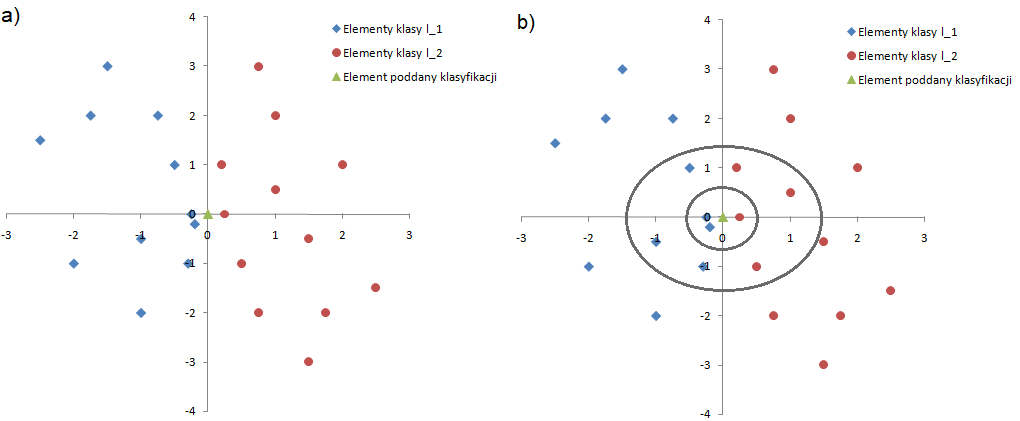
\includegraphics[scale=0.5]{kNN.PNG} 
\caption{Metoda $k$ - Najbliższych Sąsiadów.}
\end{figure}
\end{center}

Na powyższym rysunku widzimy przykładowe zastosowanie algorytmu $k$-NN. W części a) przedstawiony został zbiór treningowy z podziałem na dwie klasy (rąby, koła) oraz punkt, który będziemy chcieli przyporządkować do jednej z nich (trójkąt). W części b) przedstawiono dwa koła, jedno prezentujące najbliższe sąsiedztwo dla $k = 3$, drugie dla $k = 9$. W obu przypadkach nowy punkt (trójkąt) zostanie przyporządkowany do klasy $l_1$. Warto jednak zauważyć, że znajduje się on na granicy dwóch klastrów przez co przy innym wyborze $k$ może zostać przyporządkowany do klasy $l_2$.

Opisana metoda przyporządkowuje wybranemu rekordowi najbardziej mu podobne wykorzystując miary odległości.

Najtrudniejszym zadaniem przy przeprowadzaniu algorytmu $k$-NN jest wybór $k$. Jeżeli $k$ będzie zbyt małe - klasyfikator stanie się bardzo wrażliwy, jeżeli jednak $k$ będzie zbyt duże sąsiedztwo może zawierać zbyt dużo punktów z innych klas. Rozważając przypadek z Rysunku 3.1 łatwo zauważyć, że nawet mała zmiana w obserwacjach zbioru treningowego może doprowadzić do zmiany wyniku.

\subsection{$k$-Średnich } {\citep[Sec 2.3.1]{ascgdpds}}

Algorytm k-średnich jest prostym i zarazem efektywnym algorytmem grupowania.

Głównym celem algorytmu jest podział pewnego zbioru $X$:
$$
X = \set{x_i = (x_{i1},\ldots,x_{id}) : i \in \set{1,\ldots,N}},
$$
gdzie $x_i$ jest $d$ - wymiarowym wektorem cech opisującym obiekt na podzbiory.

W wyniku grupowania $n$ - elementowego zbioru $X$ na $k$ podgrup jest macierz podziału $A$ o wymiarach $k\times n$ . Każdy z elementów tej macierzy $a_{ik}$ oznacza stopień w jakim wektor $x_k$ przynależy do grupy. Na wstępie algorytmu ustalamy wartość parametru $k$ jako liczbę grup, które zostaną wyodrębnione. Wybieramy $k$ reprezentantów, które stanowią prototypy grup.
\begin{center}
\begin{figure}[H]
\centering
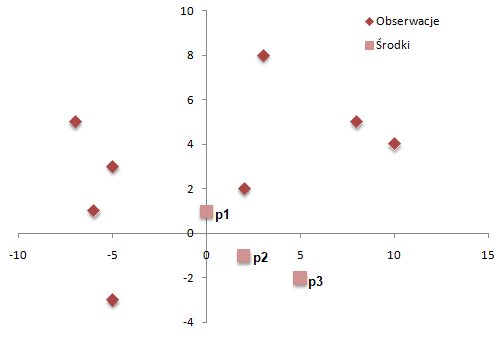
\includegraphics[scale=0.8]{ks_0.PNG} 
\caption{Metoda $k$-średnich. Wybór początkowych środków.}
\end{figure}
\end{center}

W powyższym przykładzie (Rysunek 3.2) wybranymi środkami są punkty $p1$, $p2$, $p3$. Kolejnym krokiem jest przypisanie każdego z elementów do najbliższej mu grupy.
\begin{center}
\begin{figure}[H]
\centering
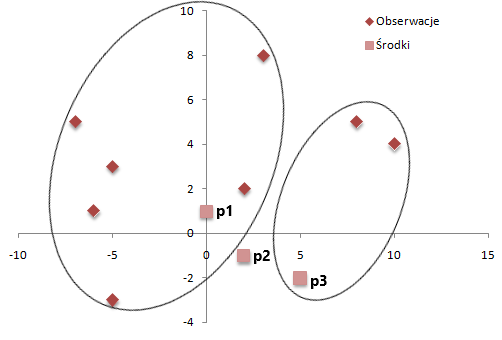
\includegraphics[scale=0.8]{ks_1.png} 
\caption{Metoda $k$-średnich. Przypisanie elementów do grup.}
\end{figure}
\end{center}
Dla każdej z tak ustalonych grup obliczamy średnią arytmetyczną współrzędnych, które staną się kolejnymi środkami.
\begin{center}
\begin{figure}[H]
\centering
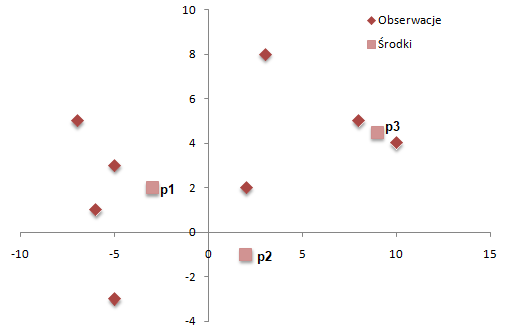
\includegraphics[scale=0.8]{ks_2.png} 
\caption{Metoda $k$-średnich. Wybór nowych środków.}
\end{figure}
\end{center}
Kroki te są wykonywane do momentu występowania migracji między obiektami.
W algorytmie $k$-średnich liczba grup pozostaje więc niezmienną, zmienna jest tylko przynależność do grup.
W metodzie tej poszukiwanie optymalnego podziału odpowiada wyznaczaniu takich grup, które minimalizują następującą funkcje kryterialną:
$$
\J{u}{B} = \sum_{i=1}^k \sum_{k=1}^N b_{ki}\distance{u_i}{x_k}^2,
$$
gdzie 
\begin{itemize}
\item $\distance{u}{x}$ oznacza odległość elementu $x$ od grupy wyznaczonej przez środek $u$,
\item $N$ to liczebność zbioru $X$,
\item $B$ oznacza macierz podziału.
\end{itemize}
 

\subsection{Maszyna Wektorów Nośnych}
Maszyny wektorów nośnych (ang. Support Vector Machines (SVM)) jest algorytmem uczenia maszynowego używanym zarówno w przypadku zadań klasyfikacji jak i regresji. Głównym celem algorytmu jest znalezienie w przestrzenie $n$ - wymiarowej hiperpłaszczyzny, która wyraźnie sklasyfikuje obserwacje i podzieli na dwie klasy maksymalizując odległość między obserwacjami. Podejście to pozwala uniknąć błędnego przyporządkowania marginalnych obserwacji w przyszłości.
\begin{center}
\begin{figure}[H]
\centering
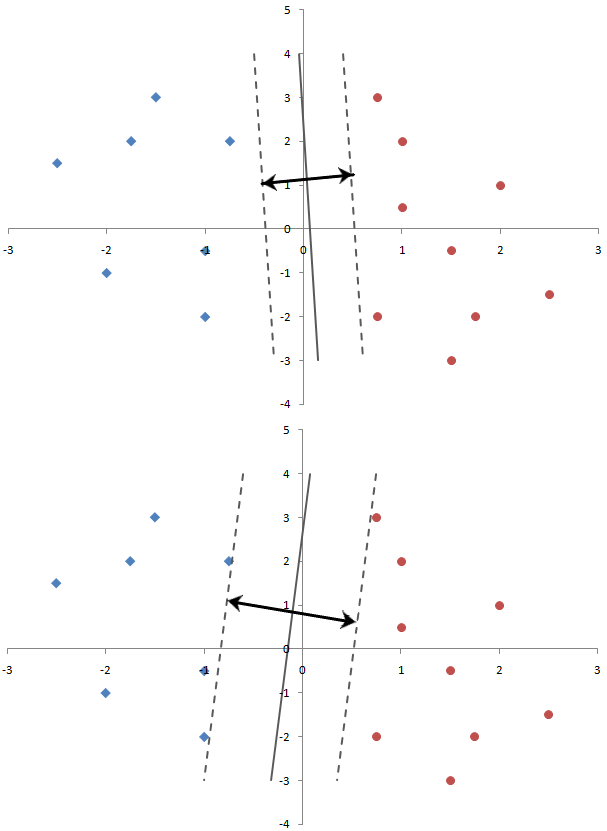
\includegraphics[scale=0.5]{SVM.PNG} 
\caption{Maszyna wektorów nośnych - maksymalizacja odległości między klasami.}
\end{figure}
\end{center}
Aby formalnie zdefiniować maszyne wektorów nośnych zacznijmy od formalnego zdefiniowania problemu klasyfikacji.
\begin{df}[Klasyfikacja {\citep{svmmwn}}]
Nich w przestrzeni $\Omega$ znajdują się wektory danych $x_i \in \setR^n$, $i\in \set{1,\ldots,n}$. $P$ niech będzie próbą uczącą.
Wtedy:
$$
P = \set{(x_i,c_i): x_i \in \setR^n, c_i \in \set{1,-1}}.
$$
\end{df}
Należy znaleźć klasyfikator dzielący całą przestrzeń $\Omega$ na dwie klasy $\{-1,1\}$, który pozwoli na przyporządkowywać nowego elementu do klasy. Szukamy funkcji $f(x)$ - granicy między klasami.

\begin{df}[Liniowa Separowalność {\citep{svmmwn}}]
Dwie klasy nazywamy liniowo separowalnymi, jeżeli istnieje hiperpłaszczyzna $\f{x}$ postaci:
$$
\f{x} = w^T x +b
$$
taka, że:
$$
\left\{\begin{array}{ll}
f(x_i)>0, &    x_i\in\set{1} \\
f(x_i)<0, &    x_i\in\set{-1}.
\end{array} \right.
$$
\end{df}
Liniową separowalność definiujemy więc za pomocą funkcji:
$$
\langle w,x \rangle + b = 0,
$$
gdzie $w, b$ są parametrami spełniającymi założenia modelu:
$$
f(x) = 
\left\{\begin{array}{lll}
1, & gdy &   \langle w,x \rangle + b > 0 \\
-1, &   gdy &   \langle w,x \rangle + b < 0.
\end{array} \right.
$$
Parametry $w$ i $b$ wyznaczamy w taki sposób, by odległość między płaszczyznami
$$
b_{i1} \: \langle w,x \rangle + b = 1,
$$
$$
b_{i2} \: \langle w,x \rangle + b = -1
$$
była maksymalna.
Zatem:
$$
\f{x} = 
\left\{\begin{array}{lll}
1, & gdy &   \langle w,x \rangle + b \geq 1 \\
-1, &   gdy &   \langle w,x \rangle + b \leq -1,
\end{array} \right.
$$
oraz szukana odległość wyznaczana jest przez maksymalizowanie funkcji:
$$
Margin=\frac{2}{\norm{w}^2}.
$$
Jest to równoważne minimalizowaniu funkcji odwrotnej:
$$
\reciprocal{W} = \frac{\norm{w}^2}{2},
$$
przy ograniczeniach
$$
y_i(\langle w,x \rangle + b) \geq 1.
$$
Problem ten nazywamy problemem optymalizacji kwadratowej i rozważamy przy użyciu mnożników Lagrange'a. 

Minimalizujemy więc funkcję Lagrange'a:
$$
\reciprocal{w,b,\alpha}=\frac{1}{2}\norm{w}^2 - \sum_{i=1}^n \alpha_i(y_i(\langle w,x \rangle + b)-1),
$$
gdzie
$\alpha_i \geq 0$ dla $i \in \set{1,...,n}$ to mnożniki Lagrange'a spełniające ograniczenia Karusha-Kuhna-Tuckera:
\begin{itemize}
\item $\alpha_i \geq 0$,
\item $\alpha_i(y_i(\langle w,x \rangle + b)-1) = 0$.
\end{itemize}

Możemy zauważyć, że w konsekwencji mnożniki Lagrange'a są niezerowe tylko dla wektorów nośnych. Liczba parametrów do oszacowania pozostaje jednak nadal zbyt duża. Częstym podejściem w tym przypadku jest przejście na postać dualną zadania optymalizacyjnego.
Maksymalizujemy tu funkcję:
$$
\sum_{i=1}^n \alpha_i - \frac{1}{2} \sum_{i=1}^n \sum_{j=1}^{n} \alpha_i \alpha_j y_i y_j(x_i \cdot x_j),
$$
przy ograniczeniach:
\begin{itemize}
\item $\alpha_i \geq 0$,
\item $\forall_i \sum_{i=1}^n \alpha_i y_i =0$.
\end{itemize}

\begin{uwaga}[{\citep{svmmwn}}]
Jeżeli elementy nie są jednak separowalne liniowo:
\begin{center}
\begin{figure}[H]
\centering
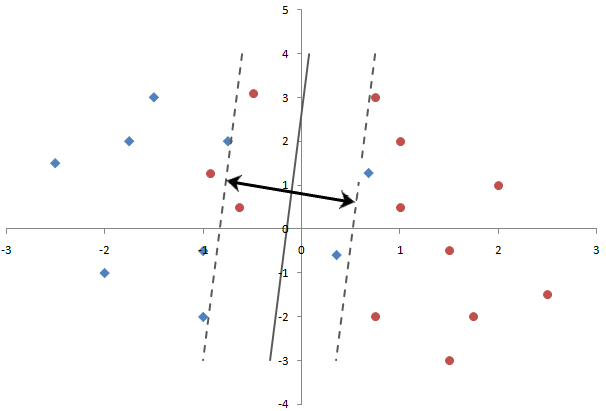
\includegraphics[scale=0.5]{SVM2.PNG} 
\caption{Maszyna wektorów nośnych - elementy nieseparowalne liniowo.}
\end{figure}
\end{center}
wprowadzamy klasyfikator Soft Margin SVM oraz zmienne osłabiające (pomocnicze).
W tym przypadku należy poddać minimalizacji funkcję:
$$
\reciprocal{W} = \frac{\norm{w}^2}{2} + C \sum_{i=1}^n \varepsilon,
$$
gdzie parametr $C$ ocenia starty związane z każdym błędnie zaklasyfikowanym punktem.
Funkcja $\f{x}$ jest natomiast dana wzorem:
$$
\f{x} = 
\left\{\begin{array}{lll}
1, & gdy &   \langle w,x \rangle + b \geq 1 - \varepsilon \\
-1, &   gdy &   \langle w,x \rangle + b \leq -1 + \varepsilon.
\end{array} \right.
$$

\end{uwaga}

Interpretacja rozwiązań:
\begin{itemize}
\item $\varepsilon_n =0$ i $\alpha_i =0$ - poprawne zaklasyfikowanie obserwacji, obserwacja leży poza marginesem,
\item $\varepsilon_n =0$ i $0<\alpha_i <C$ - poprawne zaklasyfikowanie obserwacji, obserwacja leży na jednej z płaszczyzn ograniczających margines,
\item $0<\varepsilon_n <1$ i $\alpha_i =C$ - poprawne zaklasyfikowanie obserwacji, obserwacja leży wewnątrz marginesu,
\item $\varepsilon_n \geq 1$ i $\alpha_i =C$ - niepoprawne zaklasyfikowanie obserwacji.
\end{itemize}

\section{Szacowanie błędów obliczeń}
\subsection{Ocena dokładności metody}%RecommenderSystemsHandbook
Kolejna kwestia często poruszana w regułach rekomendujących to dokładność przewidywań. Najczęściej używanymi miarami dokładności modelu są:
\begin{itemize}
\item błąd średni (Mean Error),
\item średni błąd bezwzględny (Mean Absolute Error),
\item średni błąd kwadratowy (Mean Squared Error).
\end{itemize}

Niech dla elementu $i$ ze zbioru testowego $P$ będzie dostarczona predykcja $\widehat{r}_i$. Aby ocenić jakość jej wyniku należy porównać ją ze znaną wartością $r_i$.

\begin{df}[błąd średni {\citep[Sec 4.1.1]{rsh}}]
Średnim błędem nazywamy wartość wyrażenia:
$$
ME = \frac{1}{|P|}\sum_{i\in P}(\widehat{r}_i-r_i).
$$
\end{df}

\begin{df}[średni błąd bezwzględny  {\citep[Sec 4.1.1]{rsh}}]
Średnim błędem bezwzględnym nazywamy wartość wyrażenia:
$$
MAD = \frac{1}{|P|}\sum_{i\in P}|\widehat{r}_i-r_i|.
$$
\end{df}

\begin{df}[średni błąd kwadratowy  {\citep[Sec 4.1.1]{rsh}}]
Średnim błędem kwadratowym nazywamy wartość wyrażenia:
$$
MSE = \frac{1}{|P|}\sum_{i\in P}(\widehat{r}_i-r_i)^2.
$$
\end{df}
\begin{uwaga}{\citep[Sec 4.1.1]{rsh}}
Funkcja kwadratowa jest funkcją monotoniczną co pozwala na dość częste zastępowanie średniego błędu kwadratowego przez średnią kwadratową błędów (Root Mean Squared Error (RMSE)):
$$
RMSE = \sqrt{MSE}
$$
Normalized RMSE (NRMSE) oraz Normalized MAE (NMAE) są znormalizownymi, przez użycie zakresu wartości $r_{max} - r_{min}$, wersjami błędów RMSE i MAE.
\end{uwaga}
Kolejnym rodzajem powszechnie używanego błędu, który pozwala na użycie sum ważonych jest średni błąd RMSE (Average RMSE).
\begin{df}[średni błąd RMSE {\citep[Sec 4.1.1]{rsh}}]
Niech $w_i>0$ będzie wagę dla elementu $i$ oraz niech $\sum w_i = 1$.

Średnim błędem RMSE nazywamy wartość wyrażenia:
$$
ARMSE = \sqrt{\sum_{i\in P}w_{i}(\widehat{r}_i-r_i)^2}.
$$
\end{df}
\subsection{Ocena jakości modelu}
Ocenę jakości modelu przeprowadza się na zbiorze testowym. Dla każdego z rekordów jest znana jego etykieta. Rekordy te są poddawane działaniu modelu, a następnie etykiety przypisane rekordom przez model są porównywalne z rzeczywistymi wartościami etykiet.

W następnym kroku zliczana jest liczba rekordów poprawnie i niepoprawnie zaklasyfikowanych przez model, a wynik testu zostaje przestawiony w postaci macierzy pomyłek.
\begin{df}[macierz pomyłek {\citep[Sec 4.8.1]{edmia}}]
Macierzą pomyłek nazywamy macierz kwadratową $ m \times m$ ($m$ oznacza liczbę etykiet), gdzie wiersze reprezentują etykiety początkowe, natomiast kolumny etykiety przyporządkowane rekordom przez model. Element macierzy - $f_{ij}$ oznacza liczbę rekordów z etykietą $E_i$, którym błędnie została przypisana etykieta $E_j$.
\begin{table}[H]
\begin{center}
\begin{tabular}{|r|r|r|} \hline
Etykieta przewidziana & $E_1$ & $E_2$\\
\hline
Etykieta rzeczywista & &  \\
\hline 
$E_1$ & $f_{11}$ & $f_{12}$ \\
\hline
$E_2$ & $f_{21}$ & $f_{22}$  \\
\hline
\end{tabular}
\end{center}
\caption{Macierz pomyłek.}
\label{tabelka}
\end{table}
\end{df}
\begin{uwaga}{\citep[Sec 4.8.1]{edmia}}
Często elementy macierzy pomyłek dla problemów klasyfikacji binarnej oznacza się symbolami : TP, TN, FN, FP. Oznaczenia te symbolizują cztery możliwe przypadki występujące w klasyfikacji binarnej. Załóżmy, że wyróżniamy klasę pozytywną (+) i negatywną (-). Wtedy :
\begin{itemize}
\item TP (ang. true - positive) - liczba pozytywnych rekordów testowych zaklasyfikowanych do klasy pozytywnej,
\item FN (ang. false - negative) - liczba pozytywnych rekordów testowych zaklasyfikowanych do klasy negatywnej,
\item FP (ang. false - positive) - liczba negatywnych rekordów testowych zaklasyfikowanych do klasy pozytywnej,
\item TN (ang. true - negative) - liczba negatywnych rekordów testowych zaklasyfikowanych do klasy negatywnej.
\end{itemize}
Macierz pomyłek przyjmuje wtedy postać:
\begin{table}[H]
\begin{center}
\begin{tabular}{|r|r|r|} \hline
Etykieta przewidziana & $+$ & $-$\\
\hline
Etykieta rzeczywista & &  \\
\hline 
$+$ & $TP$ & $FN$ \\
\hline
$-$ & $FP$ & $TN$  \\
\hline
\end{tabular}
\end{center}
\caption{Macierz pomyłek - przypadek klasyfikacji binarnej.}
\label{tabelka}
\end{table}
\end{uwaga}
Poprzez analizę macierzy pomyłek bez problemu obliczymy łączną liczbę rekordów zaklasyfikowanych poprawnie oraz rekordów przypisanych błędnie przez klasyfikator. 

Analizę zawartości macierzy można rozszerzyć o dodatkową informację - koszt błędnej klasyfikacji (ang. misclassification cost).
\begin{df}[koszt błędnej klasyfikacji {\citep[Sec 4.8.1]{edmia}}]
Oznaczmy przez $e_{ij}$ koszt błędnego zaklasyfikowania do klasy $E_j$ rekordu, który w rzeczywistości należy do klasy $E_i$.
Koszt poprawnej klasyfikacji oznaczmy przez $e_{ii}$ oraz załóżmy, że $\forall_{i}$ $ e_{ii} = 0$.
Dodatkowo niech $f_{t}$ oznacza liczbę wszystkich przykładów testowych, $f_{p}$ liczbę poprawnie zaklasyfikowanych rekordów testowych oraz $f_{p} = \sum_{i=1}^m f_{ii}$, $f_{b}$ niech natomiast oznacza liczbę błędnych klasyfikacji i $f_{b} = f_{t} - f_{p}$.

Kosztem błędnej klasyfikacji $E(f_{b})$ nazywamy sumę:
$$
E(f_{b}) = \sum_{i=1}^m \sum_{j=1}^m f_{ij} \cdot e_{ij}.
$$
\end{df}

W przypadkach, gdy błędne zaklasyfikowania rekordów nie różnią się kosztami, do oceny jakości klasyfikatora można wykorzystać miary takie jak trafność klasyfikacji (ang. accuracy) oraz błąd klasyfikacji (ang. error rat).
\begin{df}[trafność klasyfikacji {\citep[Sec 4.8.1]{edmia}}]
Trafnością klasyfikacji nazywamy stosunek liczby popranie zaklasyfikowanych rekordów testowych do łącznej liczby rekordów testowych:
$$
TR= \frac{f_p}{f_t} = \frac{\sum_{i=1}^m f_{ii}}{f_t}.
$$
\end{df}
\begin{df}[błąd klasyfikacji {\citep[Sec 4.8.1]{edmia}}]
Błędem klasyfikacji nazywamy stosunek liczby błędnie zaklasyfikowanych rekordów testowych do łącznej liczby rekordów testowych:
$$
BK = \frac{f_b}{f_t}=\frac{\sum_{i=1}^m \sum_{j=1}^m f_{ij}}{f_t}=1 - \frac{f_p}{f_t}.
$$
\end{df}
\begin{uwaga}{\citep[Sec 4.8.1]{edmia}}
Innymi miarami, które można wywnioskować bezpośrednio z macierzy pomyłek dla klasyfikacji binarnej (Tabla 3.2) są:
\begin{itemize}
\item $WTP$ - współczynnik $TP$ (czułość):
$$
WTP = \frac{TP}{TP + FN},
$$
\item $WFP$ - współczynnik $FP$:
$$
WFP = \frac{FP}{FP + TN},
$$
\item $WTN$ - współczynnik $TN$ (specyficzność):
$$
WTN = \frac{TN}{FP + TN},
$$
\item precyzja:
$$
precyzja = \frac{TP}{TP + FP},
$$
\item zwrot:
$$
zwrot = \frac{TP}{TP + FN},
$$
\item $F$-miara:
$$
F - miara = \frac{2 \cdot precyzja \cdot zwrot}{precyzja \cdot zwrot}.
$$
\end{itemize}
\end{uwaga}

\subsection{Ocena rankingów}
W poprzedniej sekcji została omówiona metoda wyboru odpowiedniego modelu klasyfikujące. Każdy z takich modeli kończy się przedstawieniem pewnej listy wyników. 

W tej części zostaną zaprezentowane metody służące do oceny otrzymanych na podstawie modelu rankingów i pomagające zapewnić odpowiedni porządek wyników. Jeżeli elementy posiadają oceny (np. użytkowników) intuicyjnym jest stworzyć ranking przez uporządkowanie tych ocen w malejący sposób. W przypadku gdy jednak nie mamy takich danych lub nie jest odpowiednie tworzenie takiego rankingu użyjemy znormalizowanej miary opartej na odległości (ang. Normalized Distance-based Performance Measure (NDPM): 
\begin{df}[miara znormalizowana oparta na odległości {\citep[Sec 2.2.1]{kidzinski}}]
Niech $r_{ui}$ będzie rankingiem odniesienia i $\widehat{r}_{ui}$ rankingiem stworzonym przez wybrany system rekomendujący $n_u$ elementów $i$ użytkownikowi $u$. 
Ponadto niech:
$$
C^{+} = \sum_{i<j} \sgn{r_{ui} - r_{uj}} \sgn{\widehat{r}_{ui}-\widehat{r}_{uj}}
$$
$$
C^{-} = \sum_{i<j} \sgn{r_{ui} - r_{uj}}^{2}\sgn{\widehat{r}_{uj}-\widehat{r}_{ui}}
$$
$$
C^{u} = \sum_{i<j} \sgn{r_{ui} - r_{uj}}^{2}
$$
$$
C^{s} = \sum_{i<j} \sgn{\widehat{r}_{ui}-\widehat{r}_{uj}}
$$
$$
C^{0}=C^{u}-(C^{+}-C^{-}),
$$ 
gdzie
$C^{u}$ jest liczbą par dla których ranking referencyjny okazuje się lepszą możliwością, 
$C^{+}$ i $C^{-}$ to liczba par z poprawną i niepoprawną kolejnością,
$C^{0}$ jest liczbą par dla których ranking referencyjny nie jest wiążący, kiedy ranking systemu rekomendującego jest.

Miarą NDPM nazywamy:
\begin{center}
$NDPM = \frac{C^{-} + 0.5 C^{0}}{C^{u}}$
\end{center}
\end{df}
\begin{uwaga}{\citep[Sec 2.2.1]{kidzinski}}
Powiązania w rankingu referencyjnym pojawiają się naturalnie, kiedy znamy preferencje użytkownika (np. przydziela on oceny). Czasami jednak rankingi są bardziej specyficzne (np. kiedy dajemy użytkownikowi wybór między dwoma elementami). Wtedy też system rekomendujący nie powinien tworzyć rankingu klasyfikując jedne elementy wyżej niż inne. W takich przypadkach przychodzą nam z pomocą 
\begin{itemize}
\item miara Kendall's $\tau$:
$$
\tau = \frac{C^{+} - C^{-} }{\sqrt{C^{u}}\sqrt{C^{s}}},
$$
\item miara Spearman's $\rho$:
$$
\rho = \frac{1}{n_{u}}\frac{\sum_i (r_{iu} - \overline{r})(\widehat{r}_{iu}-\overline{\widehat{r}})}{\sigma(r)\sigma(\widehat{r})},
$$
gdzie $\overline{r}$ i $\overline{\widehat{r}}$ oznaczają średnie, natomiast $\sigma(r)$ i $\sigma(\widehat{r})$ odchylenia standardowe.
\end{itemize}
\end{uwaga}



\chapter{Modele tworzenia rekomendacji}

W nieniejszym rozdziale zajmiemy się formalnym zdefiniowanie zadania, które ukrywa się pod nazwą tworzenia rekomendacji. Do jego poprawnego określenia bedą przydatne następujace pojęcia .

\begin{df}[Przedmiot {\citep[Sec 1.3]{kidzinski}}]
 Przedmiotem nazwiemy klasę obiektów tego samego typu, nierozróżnialnych dla obserwatora, reprezentowanych przez co najmniej jeden element.
\end{df}

Przedmioty stanowią podstawową grupę elementów w rozważaniach systemów rekomendujących. 

\begin{df}[Użytkownik {\citep[Sec 1.3]{kidzinski}}]
Użytkownikiem nazywamy osobę zdolną do przedstawienia własnej oceny wybranego przedmiotu.
\end{df}

W pracy \citep{kidzinski} użyty jest zawsze ten sam zbiór ocen, jednak łatwo możemy pokusić się o jego uogólnienie.

\begin{df}[Zbiór ocen {\citep[Sec 1.3]{kidzinski}}]
Podzbiór skończony zbioru $\setN$ lub $\setN \cup \set{0}$ nazywamy zbiorem ocen dla przedmiotów. 
\end{df} 

\begin{df}[Macierz preferencji {\citep[Sec 1.3]{kidzinski}}]
Rozważmy zbiór przedmiotów o liczności $n$ oraz grupę użytkowników o liczności $m$. Macierzą preferencji $M$ nazwiemy macierz o wymiarach $n \times m$ i wartościach w ustalonym zbiorze ocen.
\end{df}

Z uwagi na to, że przedmioty jako wytwory świata rzeczywistego, niemożliwe do opisania za pomocą skończonej liczby cech. Rozważa się więc ich skończoną reprezentację nazywaną wektorem własności.

\begin{df}[Własność {\citep[Sec 1.3]{kidzinski}}]
Własnością nazwiemy cechę wyrażoną za pomocą wartości liczbowej lub pewnej zmiennej kategorycznej, która reprezentuje cechę przedmiotu istotną dla użytkownika w procesie tworzenia oceny. Zbiór wszystkih własności w rozważanym modelu oznaczamy $P$. Dla każdej $p \in P$ poprzez $V_p$ rozumiemy zbiór wszystkich dopuszczalnych wartości własności $p$.
\end{df}

\begin{df}[Funkcja anotująca {\citep[Sec 1.3]{kidzinski}}]
Funkcją anotującą własność $p \in P$ nazwiemy funkcję 
$$
a_p \colon S \to V_p,
$$
gdzie $S$ oznacza zbiór wszystkich przedmiotów.
\end{df}

Mając na uwadze, że zbiór $P$ jest skończony (jak również zbiór $S$) można utożsamiać funkcję anotującą z wektorem o długości $|P|$ nazywanym wektorem własności.

\begin{df}[Problem tworzenia rekomendacji {\citep[Sec 1.3]{kidzinski}}]
Rozważmy pewien zbiór przedmiotów $S$ oraz pewien zbiór użytkowników $U$ oraz pewien zbiór ocen $Z$. Niech ponadto $R$ będzie funkcją działającą $ R: S \times U \to Z$. Załóżmy, że dla funkcji $R$ znane są wartości dla pewnych par przedmiotów i użytkowników. Zadaniem naszym jest zaproponowanie sposobu predykcji wartości tej funkcji $R$ dla brakujących par w sposób minimalizujący wybrany funkcjonał błędu. 
\end{df}

Przyjrzyjmy się następującemu przykładowi, który wykorzystamy do ilustracji tej sytuacji.

\begin{przyklad}
Załóżmy, że mamy zbiór sześciu książek $\{s_1, s_2, s_3, s_4, s_5, s_6\}$, oraz zbiór sześciu czytelników $\{u_1, u_2, u_3, u_4, u_5, u_6\}$.
Poniższa tabela przedstawia oceny jakie czytelnicy przyporządkowali po przeczytaniu poszczególnym pozycjom. Znak '?' oznacza, że czytelnik danej książki nie czytał lub czytał lecz jej nie ocenił.
\begin{center}
\begin{tabular}{|r|r|r|r|r|r|r|r|} \hline
\textbf{Czytelnicy} & & $\mathbf{u_1}$ & $\mathbf{u_2}$ & $\mathbf{u_3}$ & $\mathbf{u_4}$ & $\mathbf{u_5}$ & $\mathbf{u_6}$ \\
\hline
\hline
\textbf{Książki} &$\mathbf{s_1}$ & 6 & 3 & \textbf{?} & 6 & 4 & \textbf{?} \\
\hline
&$\mathbf{s_2}$ & \textbf{?} & 6 & 6 & 5 & 6 & \textbf{?} \\
\hline
&$\mathbf{s_3}$ & 7 & 7 & 8 & 7 & 8 & 9  \\
\hline
&$\mathbf{s_4}$ & 8 & 10 & 10 & 7 & 6 & 8 \\
\hline
&$\mathbf{s_5}$ & 9 & 6 & 6 & 6 & 6 & \textbf{?} \\
\hline
&$\mathbf{s_6}$ & 5 & 7 & 7 & 5 & 4 & 2 \\
\hline
\end{tabular}.
\end{center}

Celem jest przewidzieć brakujące oceny w sposób minimalizujący błąd popełniany przez nasz model.
\end{przyklad}
\begin{uwaga}
Systemy rekomendujące mogą zostać podzielone na systemy oparte na kontekście i systemy oparte na samych ocenach. W pierwszym przypadku predykcja jest dokonywana na podstawie przydzielonych ocen oraz pod względem wektorów cech rozważanych elementów. Główne założenie wymaga, że jeżeli użytkownik ocenił w pewien sposób przedmiot A w przeszłości oraz przedmiot B jest podobna do A, to użytkownik będzie skłonny w podobny sposób ocenić przedmiot B. W systemach opartych na ocenach, badaniu podlegają natomiast zależności które występują między produktami, a użytkownikami. Zakłada się, że jeżeli użytkownicy A i B wykazują podobieństwo oraz użytkownik A oceni pewien przedmiot, którego użytkownik B jeszcze nie ocenił, to prawdopodobnie ocena użytkownika B będzie podobna do oceny użytkownika A.
\end{uwaga}
\section{Systemy rekomendujące oparte na treści(Content-based recommender systems):}

Systemy oparte na treści wyróżnia ukierunkowanie na spersonalizowany poziom użytkownika oraz treść produktu. 
\begin{problem}
Głównym zadaniem w tej metodzie jest scharakteryzowanie wektora cech $G$, które użytkownik ceni, a następnie zasugerowanie mu produktów, które te cechy posiadają. 
\end{problem}

Wspomniana metoda opiera się na obliczaniu podobieństw oraz wykorzystuje zadania uczenia maszynowego, takie jak klasyfikacja.
\begin{algorytm}
W typie rekomendacji opartym na treści stworzenie rekomendacji i wygenerowanie listy elementów, które mogę być odpowiednie użytkownikowi możemy przedstawić w trzech krokach:
\begin{enumerate}
\item wygenerowanie profilu produktu,
\item wygenerowanie profilu użytkownika,
\item rozpoznanie cech produktu odpowiednich dla użytkownika.
\end{enumerate}
\end{algorytm}
\begin{przyklad}
Niech poniższa tabela określa w jakim stopniu (skala 0-1) każda z książek reprezentuje cechy gatunków $g_1$, $g_2$.
\begin{center}
\begin{tabular}{|r|r|r|r|} \hline
\textbf{Gatunki} & & $\mathbf{g_1}$ & $\mathbf{g_2}$  \\
\hline
\hline
\textbf{Książki} &$\mathbf{s_1}$ & 0,9 & 0 \\
\hline
&$\mathbf{s_2}$ & 1 & 0,01  \\
\hline
&$\mathbf{s_3}$ & 0,99 & 0 \\
\hline
&$\mathbf{s_4}$ & 0,1 & 1 \\
\hline
&$\mathbf{s_5}$ & 0 & 0,9 \\
\hline
&$\mathbf{s_6}$ & 0,8 & 0,3 \\
\hline
\end{tabular}
\end{center}
Dodatkowo zakładamy, że istnieje gatunek $g_0$, którego cechy reprezentują wszystkie książki oraz dla każdej z książek $g_0=1$.
Zatem $g^{(1)}= \left[
        \begin{array}{c}
         1 \\
         0,9 \\
         0 \\
         \end{array}
      \right] $ jest wektorem cech odpowiadającym książce $s_1$, $g^{(2)}= \left[
        \begin{array}{c}
         1 \\
         1 \\
         0,01 \\
         \end{array}
      \right] $ jest wektorem cech odpowiadającym książce $s_2$. Analogicznie możemy wyznaczyć podobne wektory dla każdej z książek. Należy jednak zaznaczyć, że liczba wybranych przez nas cech to $n=2$.

Dla każdego użytkownika $j$ wyznaczamy wektor parametrów $\Theta^{(j)} \in \setR^3$ (w ogólnej postaci $\Theta^{(j)} \in\setR^{n+1})$, który przedstawia (w skali 0-5) preferencje użytkownika dotyczące poszczególnych gatunków. I tak odpowiednio $\Theta^{(1)}$ to wektor preferencji czytelnika $u_1$, $\Theta^{(2)}$ wektor preferencji użytkownika $u_2$, $\Theta^{(3)}$ wektor preferencji użytkownika $u_3$ i $\Theta^{(4)}$ wektor preferencji użytkownika $u_4$, $\Theta^{(5)}$ wektor preferencji użytkownika $u_5$ i $\Theta^{(6)}$ wektor preferencji użytkownika $u_5$

Aby przewidzieć ocenę jaką użytkownik $j$ wystawiłby książce $i$ po jej przeczytaniu użyjemy równania:
\begin{center}
$(\Theta^{(j)})^T g^{(i)}$.
\end{center}
\bigskip
Obliczmy ocenę jaką książce $k_3$ wystawiłby użytkownik $u_1$ przy założeniu, że wektor preferencji użytkownika $u_1$ jest postaci $\Theta^{(j)}= \left[
        \begin{array}{c}
         0 \\
         5 \\
         0 \\
         \end{array}
      \right] $. Użytkownik ten preferuje więc książki gatunku $g_1$, gdy książki gatunków $g_0$ i $g_2$ są dla niego nieatrakcyjne.
Zatem:
\begin{center}
$(\Theta^{(1)})^T g^{(3)} = [0,5,0] \left[
        \begin{array}{c}
         1 \\
         0,99 \\
         0 \\
         \end{array}
      \right] = 0 \cdot 1 + 5 \cdot 0,99 + 0 \cdot 0 = 4,95$.
\end{center}
Przewidywaną oceną jest zatem $4,95$. Po przeprowadzeniu podobnych obliczeń dla wszystkich wcześniej nieznanych ocen możemy zarekomendować naszemu użytkownikowi nową lekturę.
\end{przyklad}
\subsection{Wygenerowanie profilu produktu - algorytm TF-IDF}
W większość systemów rekomendacji opartych na treści można zauważyć użycie prostych modeli wyszukujących. Jednym z najbardziej popularnych jest model przestrzeni wektorowej (\textit{ang. Vector Space Model}) z algorytmem TF-IDF (\textit{ang. TF – term frequency, IDF - inverse document frequency}).

\begin{df}[Model przestrzeni wektorowej {\citep[Sec 3.3.1.1]{rsh}}]
Modelem przestrzeni wektorowej nazywamy formę reprezentacji dokumentów, gdzie dokument $i$ jest reprezentowany przez wektor $x_{i}$ w przestrzeni $n$-wymiarowej, a każdy z $n$ wymiarów stanowi rozważaną cechę produktu. 
\end{df}

\begin{uwaga}
Dla danych w formie dokumentów tekstowych cechami, które pomagają scharakteryzować temat dokumentu, np. artykułu na stronie internetowej są słowa. Dla każdego ze słów zostaje obliczona wartość funkcji TFIDF (została ona dokładnie omówiona poniżej). W końcowym etapie słowa, które otrzymały najwyższe wyniki zostają uznane za charakteryzujące rozważany dokument.
Formalnie rzecz ujmując każdy z dokumentów jest przedstawiony za pomocą wektora wag, gdzie waga w odpowiedni sposób wyraża zależność między dokumentem, a badanym terminem.
\end{uwaga}

\begin{df}[TFIDF {\citep[Sec 3.3.1.1]{rsh}}]
Niech $ S = \set{s_1, s_2, \ldots ,s_n}, n\in \setN$ będzie zestawem dokumentów / analizowanych przedmiotów. Natomiast 
$G = \set{g_1, g_2, \ldots ,g_n}, \\ n\in \setN $ zestawem cech rozważanych w przedmiotach. Każdy z dokumentów $s_j, \\ j\in\set{1,\ldots,n} $ jest reprezentowany jako wektor w przestrzeni wektorowej n-wymiarowej. Zatem $ s_j = [w_{1j}, w_{2j},...,w_{nj}] $, gdzie $ w_{kj} $ jest wagą dla cechy $ g_k $ w dokumencie  $ s_j $.

TFIDF nazywamy funkcję:
$$
TFIDF(t_k, d_j) = TF(g_k, k_j) \cdot IDF,
$$
gdzie:
\begin{itemize}
\item $TF(g_k, k_j) $ (macierz \textit{term frequency}) przedstawia odniesienie każdego z podanych terminów do każdego z badanych elementów:
$$
TF(g_k, k_j)=\frac{f_{k,j}}{\max_{z}f_{z,j}},
$$
$\max_{z}f_{z,j}$ - maksymalna w odniesieniu do wszystkich cech $c_z$, które pojawiły się w dokumencie $p_j$ częstotliwość wystąpień ($f_{z,j}$) 

\item $IDF$ (\textit{inverse dokument frequency}) wyraża się formułą:
$$
IDF = \log \frac{N}{n_k}
$$
$N$ - całkowita liczba dokumentów w zbiorze,
$n_k$ - liczba dokumentów w których cecha $c_k$ wystąpiła przynajmniej raz.
\end{itemize}
Ponadto w związku z założeniem o normalizacji wagi, które zostały uzyskane w wyniku 
$TFIDF(t_k, d_j)$ poddane zostaną metodzie transformacji kosinusowej: 
$$
w_{k,j} = \frac{TFIDF(t_k, d_j)}{\sqrt{ \sum_{i=1}^{|T|}{TFIDF(t_i, d_j)}^2}}.
$$
Tak wygenerowany został zbiór słów, które są reprezentacją danego dokumentu oraz jego tematu.
\end{df}

Przy stosowaniu algorytmu $TFIDF$ zakładamy, że:
\begin{itemize}
\item rzadkie cechy są równie istotne jak częste (założenie IDF),
\item kilkukrotne wystąpienie terminu w rozważanym dokumencie jest równie istotne jak pojedyncze (założenie TF),
\item długość dokumentu (filmu, książki) nie ma znaczenia (założenie normalizacji).  
\end{itemize}
Zatem jeżeli termin występuje często w konkretnym przedmiocie rozważań (TF) i równocześnie rzadko w pozostałych elementach zboru (IDF) ma większe prawdopodobieństwo stać się jedną z istotnych cech rozważanych w temacie. Ponadto normalizacja wektorów wag pozwala zrównoważyć wartość wyników i umożliwia ich porównywanie w dalszej analizie.

\begin{uwaga}{\citep[Sec 3.3.1.1]{rsh}}
Ostatnim krokiem przed zarekomendowaniem pozycji czytelnikom jest wyestymowanie podobieństw występujących między poszczególnymi dokumentami. Naturalnymi miarami odległości, które można tu wykorzystać są:
\begin{itemize}
\item współczynnik Jaccarda mierzący odległość między zbiorami słów,
\item podobieństwa kosinusów mierzące odległość między wektorami.
Przy estymowaniu odległości kosinusów między dwoma dokumentami elementami wektora są słowa, które zostały wybrane na podstawie wcześniej przeprowadzonego algorytmu. W wektorze tym wartość $1$ oznacza, że słowo pojawiło się w zbiorze opisującym dokument, natomiast $0$ oznacza sytuację przeciwną.
\end{itemize}
\end{uwaga}
\subsection{Wygenerowanie profilu użytkownika}
Przy generowaniu wektora opisującego rozważane dokumenty należy uwzględnić komponenty opisujące preferencje użytkowników. Dla każdego użytkownika $u$ przedstawiamy jego preferencje w postaci wektora $x_u$, gdzie użytkownik pozycjonuje element $i$ poprzez wektor cech $x_i$.
\subsection{Rozpoznanie cech produktu odpowiednich dla użytkownika} 
Proces rekomendacji bazuje na dopasowaniu cech profilu użytkownika i wartości opisujących treść obiektu. Rezultatem jest stwierdzenie czy rozważany kandydat jest zainteresowany analizowanym przedmiotem. Zainteresowanie użytkownika danym przedmiotem można wyestymować używając podobieństwa cosinusów. Rozważmy dokument, gdzie użytkownik wyraża zainteresowanie większością cech w wektorze $x_i$ opisującym dokument $i$. Otrzymamy cosinus kąta między użytkownikiem i dokumentem będący dodatnim ułamkiem. Oznacza to, że kąt będzie bliski $0^{o}$ a tym samym odległość między wektorami będzie mała. W przypadku przeciwnym otrzymamy cosinus bliski zeru lub mniejszy od zera, oznacza to kąt należący do przedziału $(90^{o};180^{o})$ oraz małe podobieństwo między rozważanymi wektorami.




\section{Filtrowanie kolaboratywne (Collaborative filtering)}
Podejście kolaboratywne omija niektóre ograniczenia występujące w metodach kontekstowych. Rekomendację są dokonywane tylko na podstawie ocen. Dzięki temu systemowi możemy również dokonywać rekomendacji na przestrzeni kilku kontekstów, co pozwala uniknąć nam konkretne wyspecjalizowanej przestrzeni obecnej w metodach kontekstowych.

Wyróżniamy dwa podstawowe typy filtrowania kolaboratywnego:
\begin{itemize}
\item filtrowanie kolaboratywne oparte na użytkowniku (ang. user-based),
\item filtrowanie kolaboratywne oparte na  elementach (ang. item-based).
\end{itemize}

\subsection{Filtrowanie kolaboratywne oparte na użytkowniku}

\begin{algorytm}
Stworzenie rekomendacji filtrowania kolaboratywnego opartej na użytkowniku wykonamy w dwóch krokach:
\begin{enumerate}
\item Znalezienie podobieństwa między czytelnikami opierającego się na znanych informacjach. Najczęstszymi stosowanymi podejściami do obliczania szukanego podobieństwa są Metryka Euklidesowa i Współczynnik Korelacji Pearsona.
\item Wyestymowanie ocen, które użytkownicy (w szczególności osoba dla której tworzymy rekomendację) mogliby wystawić dla nieocenionych przez nich elementów z rozważanego zbioru.
\end{enumerate}
\end{algorytm}

W celu dokładniejszego zrozumienia wróćmy do przykładu.
\begin{przyklad}
Chcąc obliczyć podobieństwo między użytkownikiem $u_2$ i $u_3$ wybierzmy książki, które przeczytali obaj użytkownicy. W tym przypadku są to: $s_2$, $s_3$, $s_4$, $s_5$, $s_6$. Na tej podstawie tworzymy odpowiednio wektory ocen użytkowników $o_{2,3} ^{(2)}$ i $o_{2,3}^{(3)}$. 
Zatem
$$
o_{2,3} ^{(2)}= \left[
        \begin{array}{c}
         6 \\
         7 \\
         10 \\
         6 \\
         7 \\
         \end{array}
      \right] \wedge o_{2,3}^{(3)} = \left[
        \begin{array}{c}
         6 \\
         8 \\
         10 \\
         6 \\
         7 \\
         \end{array}
      \right].
$$
Posługując się odległością euklidesową
$$
d_{e}(x,y) = \sqrt{\sum_{i=1}^n \mid x_{i} - y_{i} \mid ^2 }
$$
obliczamy odległość między użytkownikami $u_2$ i $u_3$: 
$$
d_{e}(o_{2,3}^{(2)},o_{2,3}^{(3)}) = \sqrt{(6-6)^2 + (7-8)^2 + (10-10)^2 + (6-6)^2 + (7-7)^2} = \sqrt{1} = 1.
$$
Postępując w podobny sposób dla każdej z par użytkowników otrzymamy następującą macierz odległości:
\begin{center}
\begin{tabular}{|r|r|r|r|r|r|r|} \hline
\textbf{Czytelnicy} & $\mathbf{u_1}$ & $\mathbf{u_2}$ & $\mathbf{u_3}$ & $\mathbf{u_4}$ & $\mathbf{u_5}$ & $\mathbf{u_6}$ \\
\hline
$\mathbf{u_1}$ & 0 & 5,099 & 4,243 & 3 & 4,359 & 3,606 \\
\hline
$\mathbf{u_2}$ & 5,099 & 0 & 1 & 4,796 & 5,196 & 5,745 \\
\hline
$\mathbf{u_3}$ & 4,243 & 1 & 0 & 3,873 & 5 & 5,477 \\
\hline
$\mathbf{u_4}$ & 3 & 4,796 & 3,873 & 0 & 2,828 & 3,742  \\
\hline 
$\mathbf{u_5}$ & 4,359 & 5,196 & 5 & 2,828 & 0 & 3 \\
\hline 
$\mathbf{u_6}$ & 3,606 & 5,745 & 5,477 & 3,742 & 3 & 0  \\
\hline 
\end{tabular}.
\end{center}
W celu uzyskania wartości z przedziału $[0,1]$ poddajemy macierz normalizacji 
\\($max\{0,1,2,3,4,5,6,7,8,9,10\} - min\{0,1,2,3,4,5,6,7,8,9,10\}$):
\begin{center}
\begin{tabular}{|r|r|r|r|r|r|r|} \hline
\textbf{Czytelnicy} & $\mathbf{u_1}$ & $\mathbf{u_2}$ & $\mathbf{u_3}$ & $\mathbf{u_4}$ & $\mathbf{u_5}$ & $\mathbf{u_6}$ \\
\hline
$\mathbf{u_1}$ & 0 & 0,5099 & 0,4243 & 0,3 & 0,4359 & 0,3606 \\
\hline
$\mathbf{u_2}$ & 0,5099 & 0 & 0,1 & 0,4796 & 0,5196 & 0,5745 \\
\hline
$\mathbf{u_3}$ & 0,4243 & 0,1 & 0 & 0,3873 & 0,5 & 0,5477 \\
\hline
$\mathbf{u_4}$ & 0,3 & 0,4796 & 0,3873 & 0 & 0,2828 & 0,3742 \\ 
\hline 
$\mathbf{u_5}$ & 0,4359 & 0,5196 & 0,5 & 0,2828 & 0 & 0,3 \\
\hline 
$\mathbf{u_6}$ & 0,3606 & 0,5745 & 0,5477 & 0,3742 & 0,3 & 0 \\ 
\hline 
\end{tabular}.
\end{center}
Im większa odległość między czytelnikami tym mniejsze jest podobieństwo jakie między nimi występuje.
Zakładając, że największa wartość prawdopodobieństwa to $1$ macierz podobieństwa przyjmuje wartości:
\begin{center}
\begin{tabular}{|r|r|r|r|r|r|r|} \hline
\textbf{Czytelnicy} & $\mathbf{u_1}$ & $\mathbf{u_2}$ & $\mathbf{u_3}$ & $\mathbf{u_4}$ & $\mathbf{u_5}$ & $\mathbf{u_6}$ \\
\hline
$\mathbf{u_1}$ & 1 & 0,4901 & 0,5757 & 0,7 & 0,5641 & 0,6394 \\
\hline
$\mathbf{u_2}$ & 0,4901 & 1 & 0,9 & 0,5204 & 0,4804 & 0,4255 \\
\hline
$\mathbf{u_3}$ & 0,5757 & 0,9 & 1 & 0.6127 & 0,5 & 0,4523 \\
\hline
$\mathbf{u_4}$ & 0,7 & 0,5204 & 0.6127 & 1 & 0,7172 & 0,6258 \\ 
\hline 
$\mathbf{u_5}$ & 0,5641 & 0,4804 & 0,5 & 0,7172 & 1 & 0,7 \\
\hline 
$\mathbf{u_6}$ & 0,6394 & 0,4255 & 0,4523 & 0,6258 & 0,7 & 1 \\ 
\hline 
\end{tabular}.
\end{center}
Bazując na przedstawionych podobieństwach wyestymujmy ocenę jaką użytkownik $u_1$ zaproponuje dla książki $s_2$. W poniższym równaniu obliczymy średnią ważoną ocen wykorzystując wartość podobieństwa między użytkownikiem $u_1$, a pozostałymi użytkownikami, którzy wcześniej ocenili książkę:
\begin{center}
$\frac{0,4901 \cdot 6 + 0,5757 \cdot 6 + 0,7 \cdot 5 + 0,5641 \cdot 6}{0,4901 + 0,5757  + 0,7  + 0,5641} = 5,7$
\end{center}
Na podstawie metody filtrowania kolaboratywnego opartej na użytkownikach wnioskujemy, że użytkownik $u_1$ wystawiłby książce $s_2$ ocenę $5,7$.
Postępując w analogiczny sposób przewidzimy wszystkie brakujące oceny :
\begin{center}
\begin{tabular}{|r|r|r|r|r|r|r|r|} \hline
\textbf{Czytelnicy} & & $\mathbf{u_1}$ & $\mathbf{u_2}$ & $\mathbf{u_3}$ & $\mathbf{u_4}$ & $\mathbf{u_5}$ & $\mathbf{u_6}$ \\
\hline
\hline
\textbf{Książki} &$\mathbf{s_1}$ & 6 & 3 & \textbf{4,57} & 6 & 4 & \textbf{4,88} \\
\hline
&$\mathbf{s_2}$ & \textbf{5,7} & 6 & 6 & 5 & 6 & \textbf{5,72} \\
\hline
&$\mathbf{s_3}$ & 7 & 7 & 8 & 7 & 8 & 9 \\
\hline
&$\mathbf{s_4}$ & 8 & 10 & 10 & 7 & 6 & 8 \\
\hline
&$\mathbf{s_5}$ & 9 & 6 & 6 & 6 & 6 & \textbf{6,67}  \\
\hline
&$\mathbf{s_6}$ & 5 & 7 & 7 & 5 & 4 & 2 \\
\hline
\end{tabular}.
\end{center}
na których podstawie możemy dokonać rekomendacji dla naszych użytkowników.
Możemy wnioskować, że dla użytkownika $u_3$ książka $s_1$ prawdopodobnie nie będzie zbyt atrakcyjna. Użytkownik $u_6$, natomiast, z chęcią przeczyta książkę $s_5$. 
\end{przyklad}

\subsection{Filtrowanie kolaboratywne oparte na  elementach}
W przypadku filtrowania kolaboratywnego opartego na elementach wartości podobieństwa między użytkownikami zostaje zastąpiona przez  wartości podobieństwa między elementami.

\begin{algorytm}
Podobnie jak w przypadku opartym na użytkowniku, w tym również należy wykonać dwa kroki.
\begin{enumerate}
\item Pierwszym etapem jest znalezienie podobieństw występujących między elementami. Najczęstszą miarą podobieństwa w tym przypadku jest podobieństwo kosinusów. Miara ta wyraża podobieństwo miedzy n-wymiarowymi wektorami poprzez kąt między nimi w przestrzeni wektorowej. Wraz ze wzrostem wartość kąta rośnie podobieństwo.
\item Następnie, na podstawie wydanych przez użytkownika ocen, należy wyestymować noty dla elementów przez niego nieocenionych.
\end{enumerate}
\end{algorytm}

\begin{przyklad}
W tym przypadku wektory odzwierciedlają zbiory ocen wystawione poszczególnym książkom przez użytkowników.
Wektor mają zatem postać:
\begin{center}
$o^{(s_1)} = \left[
        \begin{array}{c}
         6 \\
         3 \\
         6 \\
         4 \\
         \end{array}
      \right]$, $o^{(s_2)} = \left[
        \begin{array}{c}
         6 \\
         6 \\
         5 \\
         6 \\
         \end{array}
      \right]$, $o^{(s_3)} = \left[
        \begin{array}{c}
         7 \\
         7 \\
         8 \\
         7 \\
         8 \\
         9 \\
         \end{array}
      \right]$, $o^{(s_4)} = \left[
        \begin{array}{c}
         8 \\
         10 \\
         10 \\
         7 \\
         6 \\
         8 \\
         \end{array}
      \right]$, $o^{(s_5)} = \left[
        \begin{array}{c}
         9 \\
         6 \\
         6 \\
         6 \\
         6 \\
         \end{array}
      \right]$, $o^{(s_6)} = \left[
        \begin{array}{c}
         5 \\
         7 \\
         7 \\
         5 \\
         4 \\
         2 \\
         \end{array}
      \right]$
\end{center}
Warto zauważyć, że wektory są różnej długości.

Aby obliczyć podobieństwo między książkami $s_1$ i $s_2$ wyznaczmy wektory ocen w których uwzględnimy przypadki, gdzie jeden użytkownik ocenił obie pozycje.
Zatem:
\begin{center}
$\overline{o^{(s_1)}} = \left[
        \begin{array}{c}
         3 \\
         6 \\
         4 \\
         \end{array}
      \right]$, $\overline{o^{(s_2)}} = \left[
        \begin{array}{c}
         6 \\
         5 \\
         6 \\
         \end{array}
      \right]$.
\end{center}
Następnie używając wzoru na podobieństwo kosinusowe
$$
sim(\overrightarrow{a},\overrightarrow{b}) = \frac{\overrightarrow{a} \cdot \overrightarrow{b}}{|\overrightarrow{a}||\overrightarrow{b}|}
$$ 
obliczamy podobieństwo między wybranymi książkami
$$
sim(s_1,s_2) = \frac{\overline{o^{(s_1)}} \cdot \overline{o^{(s_2)}}}{|o^{(s_1)}||o^{(s_2)}|} = \frac{3 \cdot 6 + 6 \cdot 5 + 4 \cdot 6}{\sqrt{6^2 + 3^2 + 6^2 + 4^2} \sqrt{6^2 + 6^2 + 5^2 + 6^2}} = 0,6339.
$$
Postępując w analogiczny sposób otrzymamy macierz podobieństwa elementów:
\begin{center}
\begin{tabular}{|r|r|r|r|r|r|r|r|} \hline
\textbf{Czytelnicy} & $\mathbf{s_1}$ & $\mathbf{s_2}$ & $\mathbf{s_3}$ & $\mathbf{s_4}$ & $\mathbf{s_5}$ & $\mathbf{s_6}$ \\
\hline
$\mathbf{s_1}$ & 1 & 0,6339 & 0,7372 & 0,7195 & 0,8935 & 0,7599 \\
\hline
$\mathbf{s_2}$ & 0,6339 & 1 & 0,7951 & 0,8150 & 0,7977 & 0,8898 \\
\hline
$\mathbf{s_3}$ & 0,7372 & 0,7951 & 1 & 0,9780 & 0,8586 & 0,9200 \\
\hline
$\mathbf{s_4}$ & 0,7195 & 0,8150 & 0,9780 & 1 & 0,8860 & 0,9681 \\
\hline 
$\mathbf{s_5}$ & 0,8935 & 0,7977 & 0,8586 & 0,8860 & 1 & 0,9413 \\
\hline 
$\mathbf{s_6}$ & 0,7599 & 0,8898 & 0,9200 & 0,9681 & 0,9413 & 1 \\
\hline 
\end{tabular}.
\end{center}
Wyestymujmy teraz ocenę jaką użytkownik $u_6$ zaproponuje dla książki $s_2$. Ponownie obliczymy średnią ważoną ocen, tym razem, wykorzystując wartość podobieństwa między książką $k_1$, a książkami ocenionymi wcześniej przez użytkownika oraz oceny jakie nadał on tym pozycjom:
$$
\frac{(0,7951 \cdot 9 + 0,8150 \cdot 8 + 0,8898 \cdot 2)}{(0,7951 + 0,8150 + 0,8898)} = 6,16.
$$
Na podstawie przeprowadzonych obliczeń zakładamy, że ocena jaką wystawiłby po przeczytaniu użytkownik $u_6$ książce $s_2$ to $6,16$.
Powtarzając powyższe obliczenia dla każdej z pozycji wcześniej nieocenionej przez wybranego użytkownika otrzymamy wszystkie brakujące opinie. Następnie bazując na zdobytych danych z łatwością odnajdziemy pozycję najbardziej odpowiednią do zarekomendowania użytkownikowi.
\end{przyklad}
\section{Hybrydowe systemy rekomendacji}
Aby uzyskać lepsze wyniki możemy wykorzystać podczas tworzenia rekomendacji zarówno filtrowanie kolaboratywne jak i metody oparte na treści.
\bigskip
\bigskip

Niech:
\begin{itemize}
\item $n_u$ oznacza liczbę użytkowników,
\item $n_m$ oznacza liczbę elementów.
\end{itemize}
Dodatkowo wprowadźmy parametry:
\begin{itemize}
\item $r(i,j)$, gdzie $r(i,j)=1$, jeżeli użytkownik $j$ ocenił element $i$,
\item $y(i,j)$ - ocena jaką użytkownik $j$ przydzielił elementowi $i$ (ocenę definiujemy tylko wtedy gdy $r(i,j)=1$).
\end{itemize}
Znając wektory preferencji użytkowników $\Theta^{(1)}, \Theta^{(2)},\ldots,\Theta^{(n_u)}$ odnajdźmy wektor cech konkretnego elementu $g^{(i)}$, gdzie $i \in \set{1,\ldots,n_m}$?
Minimalizując następujące równanie:
$$
\min \limits_{g^{(i)}} \frac{1}{2} \sum_{j:r(i,j)=1} ((\Theta^{(j)})^T g^{(i)} - y(i,j))^2 + \frac{\lambda}{2} \sum_{k=1}^n (g_k^{(i)})^2.
$$

Aby odnaleźć wektory cech $g^{(1)}, g^{(2)},\ldots,g^{(n_m)}$ wszystkich elementów równanie, które minimalizujemy przyjmuje następującą postać:
$$
\min \limits_{g^{(1)},...,g^{(n_m)}} \frac{1}{2} \sum_{i=1}^{n_m} \sum_{j:r(i,j)=1} ((\Theta^{(j)})^T g^{(i)} - y(i,j))^2 + \frac{\lambda}{2} \sum_{i=1}^{n_m} \sum_{k=1}^n (g_k^{(i)})^2.
$$

Znając wektory cech elementów i oceny wystawione przez użytkowników możemy przewidzieć wektory preferencji użytkowników $\Theta^{(1)}, \Theta^{(2)},\ldots,\Theta^{(n_u)}$ poprzez:
$$
\min \limits_{\Theta^{(1)}, \Theta^{(2)},\ldots,\Theta^{(n_u)}} \frac{1}{2} \sum_{i=1}^{n_u} \sum_{j:r(i,j)=1} ((\Theta^{(j)})^T g^{(i)} - y(i,j))^2 + \frac{\lambda}{2} \sum_{i=1}^{n_u} \sum_{k=1}^n (\Theta^{(j)})^2.
$$
Ponownie znając $\Theta^{(1)}, \Theta^{(2)},\ldots,\Theta^{(n_u)}$ możemy wyestymować $g^{(1)}, g^{(2)},\ldots,g^{(n_m)}$.

Powtarzając powyższe kroki odnajdowania wektorów cech elementów i wektorów preferencji użytkowników stworzymy algorytm, który z każdą iteracją będzie dokładniej estymował szukane wartości.
\section{Systemy rekomendujące kontekstowe ( Context – aware recommender systems):}

Systemy rekomendujące kontekstowe są systemami rekomendującymi opartymi na treści w których zostaje uwzględniony dodatkowy wymiar zwany kontekstem. Uprzednio opisane metody opierały się głownie na rozważaniu problemów dwu-wymiarowych. W tym podejściu, przez dodanie nowego wymiaru, jakim jest kontekst $(K)$, zaczynamy rozważać problemy trój-wymiarowe:
$$
R: U \times S \times K  \rightarrow Z
$$
\begin{df}[Kontekst {\citep[Sec 3.3.1.1]{rsh}}]
Kontekstem nazywamy wektor preferencji.
\end{df}

\begin{algorytm}
W modelu kontekstowym rekomendacje są generowane w dwóch krokach:
\begin{enumerate}
\item Metody systemów rekomendujących opartych na treści służące do wygenerowania listy rekomendacji bazującej na  preferencjach użytkownika.
\item Odfiltrowanie rekomendacji, które odpowiadają przyjętemu kontekstowi.
Wyróżniamy tutaj dwa warianty. W pierwszym etap filtrowania zostaje dokonany na końcu, natomiast w drugim filtrowanie jest etapem wstępnym do tworzenia rekomendacji.


Filtrowanie jako etap wstępny (ang. Pre-Filtering)
W tym podejściu informacje kontekstowe używane są do odfiltrowania najbardziej istotnych informacji i skonstruowania dwuwymiarowego zbioru danych. Bardzo dużą zaletą tego podejścia jest możliwość implementacji w kolejnym kroku wcześniej opisanych metod rekomendacji. 

Filtrowanie jako etap końcowy (ang. Post-Filtering)
Informacje o kontekście są ignorowane w wejściowych danych, a rekomendacja dokonywana jest na całym zbiorze. To w następnym kroku lista rekomendacji stworzona dla użytkownika jest zawężana przez uwzględnienie kontekstu.
\end{enumerate}
\end{algorytm}

\chapter{Eksperymenty / cześć praktyczne}
\section{Faktoryzacja macierzy w regułach rekomendujących}
Rozważany problem rekomendacji może być sformułowany jako problem uczenia maszynowego w którym znane są oceny jakie użytkownicy wystawili pewnym przedmiotom i którego zadaniem jest predykcja ocen użytkowników dla elementów przez nich nieocenionych. 

Załóżmy, że mamy $n$ użytkowników i $m$ elementów. Otrzymujemy $n \times m$ - wymiarową macierz $R$, w której wyraz $r_{ui}$ jest oceną wystawioną przez użytkownika $u$ elementowi $i$, $i \in \set{1, \ldots, m}$. Naszym celem jest wypełnić macierz $R$ brakującymi ocenami. 

W przypadku filtrowania kolaboratywnego znaną metodą rozwiązania takiego problemu jest faktoryzacja macierzy.

\begin{df}[Faktoryzacja macierzy {\citep{mcvals}}]
Faktoryzacją macierzy nazywamy rozkład macierzy na produkt macierzy.  
\end{df}

W kontekście rekomendacji algorytm faktoryzacji macierzy działa przez dekompozycję macierzy $R$ w produkt dwóch  macierzy $X$ i $Y$. $X$ jest macierzą użytkowników (wiersze reprezentują poszczególnych użytkowników), natomiast macierz $Y$ to macierz elementów (kolumny oznaczają elementy).

\begin{df}[Postać macierzowa faktoryzacji macierzy {\citep{mcvals}}]
Niech $x_1, \ldots , x_n \in \setR ^k$ będą faktorami użytkowników oraz $y_1, \ldots, y_m \in \setR^k$ będą faktorami elementów. Wtedy $k \times n$ - wymiarowa macierz użytkowników $X$ oraz $k \times m$ - wymiarowa macierz elementów $Y$ mają następujące postaci:
$$
X = \left[
        \begin{array}{ccc}
         | & & | \\
         x_1 & \ldots & x_n \\
         | & & | \\
         \end{array}
      \right],
$$
$$
Y = \left[
        \begin{array}{ccc}
         | & & | \\
         y_1 & \ldots & y_m \\
         | & & | \\
         \end{array}
      \right].
$$      
\end{df}

\section{ALS z Apache Spark i MLlib}
\subsection{Apache Spark}
Apache Spark to ciesząca się ostatnio dużą popularnością platforma obliczeniowa stworzona w celu przetwarzania dużych zbiorów danych (BigData). Powstała ona w odpowiedzi na platformę MapReduce wykorzystywaną przez Apache Hadoop. Wspomniany MapReduce przetwarza dane w trybie wsadowym co oznacza, że podczas każdej operacji są one wczytywane i zapisywane na dysku (HDFS) przez co spada znacznie jego wydajność przy algorytmach iteracyjnych. W przypadku Apache Spark i głównej jego idei jaką jest 
Resilient Distributed Dataset zbiory danych są wczytywane do pamięci i dzięki temu są wykorzystywane przez kolejne kroki algorytmu bez konieczności ponownego wczytywania ich na dysk. Zwiększa to znacznie wydajność i szybkość wykonywania operacji.

Jedną z głównych bibliotek Apache Spark jest biblioteka MLlib. Jest to biblioteka uczenia maszynowego, której celem jest uczynić je łatwym i skalowalnym. MLLib zapewnia narzędzia do obsługi algorytmów klasyfikacji, regresji, klastrowania, redukcji wymiaru, narzędzia algebry liniowej, statystyki i wiele innych. Biblioteka ta wspiera również narzędzia do obsługi reguł rekomendujących, a w szczególności filtrowania kolaboratywnego.

\subsection{ALS i MLlib}
Alternating Least Square (ALS) jest algorytmem faktoryzacji macierzy, który został zaimplementowany bibliotece uczenia maszynowego MLlib należącej do Apache Spark. Algorytm ten został opracowany z myślą o rozwiązywaniu problemów filtrowania na dużą skalę. Jest prosty a zarazem dobrze skalowalny w stosunku do dużych zbiorów danych.

Problem predykcji brakujących ocen formułujemy jako problem optymalizacyjny, gdzie celem jest zminimalizowanie funkcji celu oraz odnalezienie najbardziej optymalnych macierzy $X$ i $Y$. 

W szczególności staramy się zminimalizować błąd najmniejszych kwadratów postaci {\citep{mcvals}}:
$$
\min_{X,Y} \sum_{r_{ui}} (r_{ui} - x_u^Ty_i)^2 + \lambda (\sum_u \norm{x_u}^2 + \sum_i \norm{y_i}^2),
$$
gdzie 
\begin{itemize}
\item $r_{ui}$ są znanymi ocenami wystawionymi przez użytkowników,
\item $\lambda$ jest czynnikiem regulującym.
\end{itemize}

Powyższa funkcja nie jest funkcją wypukłą (ze względu na obiekt $x_u^Ty_i$). Ustalając jednak jedną z macierzy $X$ lub $Y$, otrzymujemy postać kwadratową, którą można rozwiązać. Rozwiązanie zmodyfikowanego problemu gwarantuje monotoniczne obniżenie ogólnej funkcji kosztów. Stosując ten krok naprzemiennie do macierzy $X$ i $Y$, możemy iteracyjnie poprawiać faktoryzację macierzy. Podejście to określamy jako algorytm ALS (Alternating Least Squares).

\begin{algorytm}[ALS {\citep{mcvals}}]
Zainicjowanie X, Y.

Powtarzamy:
\begin{itemize}
\item for $u = 1, \ldots, n $ wykonujemy: 
$$
x_u = (\sum_{r_{ui} \in r_{u*}} y_i y_i^T + \lambda I_k)^{(-1)} \sum_{r_{ui} \in r_{u*}} r_{ui}y_i
$$
koniec for
\item for $i = 1, \ldots, m$ wykonujemy:
$$
y_i = (\sum_{r_{ui} \in r_{*i}} x_u x_u^T + \lambda I_k)^{(-1)} \sum_{r_{ui} \in r_{*i}} r_{ui}x_u
$$
koniec for
\end{itemize}
do momentu zbieżności.
\end{algorytm}
\subsection{Implementacja algorytmu}
\chapter{Podsumowanie}
%TODO napiszemy na koncu



\nocite{*} %TODO remove
\bibliographystyle{plain}
\bibliography{bibliografia}
\end{document}
